\documentclass[english,submission]{programming}
%DIF LATEXDIFF DIFFERENCE FILE
%DIF DEL diff/old-prog22.tex   Wed Sep 28 15:12:55 2022
%DIF ADD diff/new-prog22.tex   Wed Sep 28 15:06:15 2022

%\citestyle{acmauthoryear}
%\markboth{}{}

% Class scrartcl Warning: seems someone has broken package `auxhook'.
% Usually this happens, if `auxhook' is loaded or used implicitly or explicitly
% by patching \document or via etoolbox command \AtEndPreamble. Trying an
% emergency workaround. You can avoid this warning adding:
\usepackage{auxhook}
% before \begin{document} on input line 6.
\usepackage{changepage} % For the single-page summary table PDF insert.
\usepackage{pdfpages}
\usepackage{pifont} % For checkmark / cross symbols for Appendix table :)
%DIF 15a15-16
\usepackage{amsthm} % For numberless Definition %DIF > 
\usepackage{epigraph} % For the opening quotes %DIF > 
%DIF -------

% Thanks https://tex.stackexchange.com/a/32687
\NewDocumentCommand{\rot}{O{45} O{1em} m}{\makebox[#2][l]{\rotatebox{#1}{#3}}}%
%DIF PREAMBLE EXTENSION ADDED BY LATEXDIFF
%DIF UNDERLINE PREAMBLE %DIF PREAMBLE
\RequirePackage[normalem]{ulem} %DIF PREAMBLE
\RequirePackage{color}\definecolor{RED}{rgb}{1,0,0}\definecolor{BLUE}{rgb}{0,0,1} %DIF PREAMBLE
\providecommand{\DIFadd}[1]{{\protect\color{blue}\uwave{#1}}} %DIF PREAMBLE
\providecommand{\DIFdel}[1]{{\protect\color{red}\sout{#1}}}                      %DIF PREAMBLE
%DIF SAFE PREAMBLE %DIF PREAMBLE
\providecommand{\DIFaddbegin}{} %DIF PREAMBLE
\providecommand{\DIFaddend}{} %DIF PREAMBLE
\providecommand{\DIFdelbegin}{} %DIF PREAMBLE
\providecommand{\DIFdelend}{} %DIF PREAMBLE
\providecommand{\DIFmodbegin}{} %DIF PREAMBLE
\providecommand{\DIFmodend}{} %DIF PREAMBLE
%DIF FLOATSAFE PREAMBLE %DIF PREAMBLE
\providecommand{\DIFaddFL}[1]{\DIFadd{#1}} %DIF PREAMBLE
\providecommand{\DIFdelFL}[1]{\DIFdel{#1}} %DIF PREAMBLE
\providecommand{\DIFaddbeginFL}{} %DIF PREAMBLE
\providecommand{\DIFaddendFL}{} %DIF PREAMBLE
\providecommand{\DIFdelbeginFL}{} %DIF PREAMBLE
\providecommand{\DIFdelendFL}{} %DIF PREAMBLE
%DIF LISTINGS PREAMBLE %DIF PREAMBLE
\RequirePackage{listings} %DIF PREAMBLE
\RequirePackage{color} %DIF PREAMBLE
\lstdefinelanguage{DIFcode}{ %DIF PREAMBLE
%DIF DIFCODE_UNDERLINE %DIF PREAMBLE
  moredelim=[il][\color{red}\sout]{\%DIF\ <\ }, %DIF PREAMBLE
  moredelim=[il][\color{blue}\uwave]{\%DIF\ >\ } %DIF PREAMBLE
} %DIF PREAMBLE
\lstdefinestyle{DIFverbatimstyle}{ %DIF PREAMBLE
	language=DIFcode, %DIF PREAMBLE
	basicstyle=\ttfamily, %DIF PREAMBLE
	columns=fullflexible, %DIF PREAMBLE
	keepspaces=true %DIF PREAMBLE
} %DIF PREAMBLE
\lstnewenvironment{DIFverbatim}{\lstset{style=DIFverbatimstyle}}{} %DIF PREAMBLE
\lstnewenvironment{DIFverbatim*}{\lstset{style=DIFverbatimstyle,showspaces=true}}{} %DIF PREAMBLE
%DIF END PREAMBLE EXTENSION ADDED BY LATEXDIFF

\begin{document}

\paperdetails{perspective=art, area={Programming systems}}

\title{Technical Dimensions of Programming Systems}

\author{Joel Jakubovic}
\affiliation{
University of Kent, Canterbury, UK
\email{jdj9@kent.ac.uk}
}
\author{Jonathan Edwards}
\affiliation{\email{jonathanmedwards@gmail.com}}
\author{Tomas Petricek}
\affiliation{
University of Kent, Canterbury, UK
\email{T.Petricek@kent.ac.uk}
}

\keywords{Programming Systems, Dimensions, Design, Framework, Analysis}

% Please go to https://dl.acm.org/ccs/ccs.cfm and generate your Classification
% System [view CCS TeX Code] stanz and copy _all of it_ to this place.
%% From HERE
\begin{CCSXML}
<ccs2012>
   <concept>
       <concept_id>10011007.10011006.10011066.10011069</concept_id>
       <concept_desc>Software and its engineering~Integrated and visual development environments</concept_desc>
       <concept_significance>500</concept_significance>
       </concept>
   <concept>
       <concept_id>10003120.10003121.10003129</concept_id>
       <concept_desc>Human-centered computing~Interactive systems and tools</concept_desc>
       <concept_significance>300</concept_significance>
       </concept>
   <concept>
       <concept_id>10003120.10003121.10003122</concept_id>
       <concept_desc>Human-centered computing~HCI design and evaluation methods</concept_desc>
       <concept_significance>300</concept_significance>
       </concept>
 </ccs2012>
\end{CCSXML}
\ccsdesc[500]{Software and its engineering~Integrated and visual development environments}
\ccsdesc[300]{Human-centered computing~Interactive systems and tools}
\ccsdesc[300]{Human-centered computing~HCI design and evaluation methods}

\maketitle

\begin{abstract}
  \emph{Context.} Programming requires much more than just writing code in a programming language. It is usually done in the context of a stateful environment, by interacting with a system through a graphical user interface. Yet, this wide space of possibilities lacks a common structure for navigation. Work on programming systems fails to form a coherent body of research, making it hard to improve on past work and advance the state of the art.

  \emph{Inquiry.} In computer science, much has been said and done to allow comparison of \emph{programming languages}, yet no similar theory exists for \emph{programming systems;} we believe that programming systems deserve a theory too. 

  \emph{Approach.} We present a framework of \emph{technical dimensions} which capture the underlying characteristics of programming systems and provide a means for conceptualizing and comparing them. 

  \emph{Knowledge.} We identify technical dimensions by examining past influential programming systems and reviewing their design principles, technical capabilities, and styles of user interaction. Technical dimensions capture characteristics that may be studied, compared and advanced independently. This makes it possible to talk about programming systems in a way that can be shared and constructively debated rather than relying solely on personal impressions.

  \emph{Grounding.} Our framework is derived using a qualitative analysis of past programming systems. We outline two concrete ways of using our framework. First, we show how it can analyze a recently developed novel programming system. Then, we use it to identify an interesting unexplored point in the design space of programming systems. 

  \emph{Importance.} Much research effort focuses on building programming systems that are easier to use, accessible to non-experts, moldable and/or powerful, but such efforts are disconnected. They are informal, guided by the personal vision of the authors and thus are only evaluable and comparable on the basis of individual experience using them. By providing foundations for more systematic research, we can help programming systems researchers to stand, at last, on the shoulders of giants.

NOTE TO REVIEWERS: The main contribution of the paper is a comprehensive \DIFdelbegin \DIFdel{survey }\DIFdelend \DIFaddbegin \DIFadd{catalogue }\DIFaddend of 22 design dimensions of programming systems. Each one comes with detailed discussion, including known uses, to properly motivate it. \DIFdelbegin \DIFdel{Regrettably, we only have space for a small number of these dimensions }\DIFdelend \DIFaddbegin \DIFadd{We feel these belong }\DIFaddend in the main paper body \DIFdelbegin \DIFdel{. To give a broader picture of what we are contributing, we invite the reader to explore Appendix}\DIFdelend \DIFaddbegin \DIFadd{rather than in an appendix, even though this increases the page count, and have received permission to do this. We intend the catalogue as a reference to be used }\emph{\DIFadd{as necessary,}} \DIFadd{not to be read from start to finish. This means that Section}\DIFaddend \ \DIFdelbegin \DIFdel{\ref{dimensions-catalogue} for dimensions that suit their interest}\DIFdelend \DIFaddbegin \DIFadd{\ref{technical-dimensions-catalogue} can be considered to be }\textbf{\DIFadd{outside}} \DIFadd{of the normal reviewable material, leaving the rest of the paper within the journal's 22 page limit}\DIFaddend .
\end{abstract}

%\thispagestyle{empty}

\newcommand{\joel}[1]{}
\newcommand{\note}[1]{}
\newcommand{\tp}[1]{}
\newcommand{\mybox}[1]{\noindent\fbox{\parbox{\textwidth}{#1}}}
\providecommand{\tightlist}{}% Don't want Pandoc's tight lists
\DIFaddbegin \newtheorem*{defn}{Definition}
\DIFaddend %\newcommand{\hypertarget}[1]{}

\DIFdelbegin %DIFDELCMD < \begin{quote}
%DIFDELCMD < %%%
\DIFdel{A systematic presentation removes ideas from the ground that made them
grow and arranges them in an artificial pattern.
}\DIFdelend \DIFaddbegin \setlength{\epigraphwidth}{0.7\linewidth}
\epigraph{A systematic presentation removes ideas from the ground that made them grow and arranges them in an artificial pattern.}{\textit{The Tyranny of Science} \\ \textsc{Paul Feyerabend}}
\DIFaddend 

\DIFdelbegin \DIFdel{--- Paul Feyerabend, }\emph{\DIFdel{The Tyranny of Science}}%DIFAUXCMD
\DIFdel{, Polity Press (2011)
}%DIFDELCMD < \end{quote}
%DIFDELCMD < %%%
\DIFdelend \DIFaddbegin \joel{
\renewcommand{\epigraphflush}{flushleft}
\renewcommand{\sourceflush}{flushleft}
}
\DIFaddend 

\DIFdelbegin %DIFDELCMD < \begin{quote}
%DIFDELCMD < %%%
\DIFdel{Irony is said to allow the artist to continue his creative production
while immersed in a sociocultural context of which he is critical.
}\DIFdelend \DIFaddbegin \epigraph{Irony is said to allow the artist to continue his creative production while immersed in a sociocultural context of which he is critical.}{\emph{Irony; or, the Self-Critical Opacity of Postmodernist Architecture} \\ \textsc{Emmanuel Petit} }
\DIFaddend 

\DIFdelbegin \DIFdel{--- Emmanuel Petit, }\emph{\DIFdel{Irony or, the Self-Critical Opacity of
Postmodernist Architecture}}%DIFAUXCMD
\DIFdel{, Yale (2013)
}%DIFDELCMD < \end{quote}
%DIFDELCMD < 

%DIFDELCMD < %%%
\DIFdelend \hypertarget{introduction}{%
\section{Introduction}\label{introduction}}

Many forms of software have been developed to enable programming. The
classic form consists of a \emph{programming language}, a text editor to
enter source code, and a compiler to turn it into an executable program.
Instances of this form are differentiated by the syntax and semantics of
the language, along with the implementation techniques in the compiler
or runtime environment. Since the advent of graphical user interfaces
(GUIs), programming languages can be found embedded within graphical
environments that increasingly define how programmers work with the
language---for instance, by directly supporting debugging or
refactoring. Beyond this, the rise of GUIs also permits diverse visual
forms of programming, including visual languages and GUI-based end-user
programming tools. This paper advocates a shift of attention from
\emph{programming languages} to the more general notion of ``software
that enables programming''---in other words, \emph{programming systems}.

\DIFaddbegin \begin{defn}[Programming System]
\DIFaddend A \emph{programming system} \DIFdelbegin \DIFdel{may include tools , protocols, notations,
interfaces, and languages. It is a software artifact that makes it
possible to construct programs, debug them, and turn them into
operational, maintained, }\DIFdelend \DIFaddbegin \DIFadd{is an integrated and complete set of tools sufficient for creating, modifying, and executing programs. These will include notations for structuring programs and data, facilities for running and debugging programs, }\DIFaddend and \DIFdelbegin \DIFdel{evolvable artifacts running on appropriate
hardware.
}\DIFdelend \DIFaddbegin \DIFadd{interfaces for performing all of these tasks. Facilities for testing, analysis, packaging, or version control may also be present. Notations include programming languages and interfaces include text editors, but are not limited to these.
}\end{defn}

\DIFaddend This notion covers classic programming languages together with their
editors, debuggers, compilers, and other tools. Yet it is intentionally
broad enough to accommodate image-based programming environments like
Smalltalk, operating systems like UNIX, and hypermedia authoring systems
like Hypercard, in addition to various other examples we will mention.

\hypertarget{what-is-the-problem}{%
\subsection{What is the problem?}\label{what-is-the-problem}}

There is a growing interest in broader forms of \emph{programming
systems}, both in the programming research community and in industry. On
the one hand, researchers are studying topics such as \emph{programming
experience} and \emph{live programming} that require considering not
just the \emph{language}, but further aspects of a given system. On the
other hand, commercial companies are building new programming
environments like Replit~\cite{ReplitWeb} or low-code tools like
Dark~\cite{DarkWeb} and Glide~\cite{GlideWeb}. Yet, such topics remain
at the sidelines of mainstream programming research. While
\emph{programming languages} are a well-established concept, analysed
and compared in a common vocabulary, no similar foundation exists for
the wider range of \emph{programming systems}.

The academic research on programming suffers from this lack of common
vocabulary. While we may thoroughly assess programming \emph{languages},
as soon as we add interaction or graphics into the picture, \DIFdelbegin \DIFdel{we often get
stuck on how the resulting system is vaguely ``interesting'' . }\DIFdelend \DIFaddbegin \DIFadd{evaluation
beyond subjective ``coolness'' becomes fraught with
difficulty.}\footnote{\DIFadd{The same difficulty in the context of user
  interface systems has been analyzed by Olsen~\mbox{%DIFAUXCMD
\cite{EvUISR}}\hspace{0pt}%DIFAUXCMD
.
  Interesting future work would be a detailed analysis of publications
  on programming systems to understand this issue in depth. One notable
  characteristic is that publications tend to present (parts of) new
  systems. This is the case for 5/6 and 6/7 papers in the LIVE 2020 and
  2021 workshops respectively~\mbox{%DIFAUXCMD
\cite{LIVE20, LIVE21}}\hspace{0pt}%DIFAUXCMD
. In contrast,
  publications in the field of programming }\emph{\DIFadd{languages}} \DIFadd{often
  address specific issues of interest to a greater number of languages.}}
\DIFaddend Moreover, when designing new systems, inspiration is often drawn from
the same few standalone sources of ideas. These might be influential
past systems like Smalltalk, programmable end-user applications like
spreadsheets, or motivational illustrations by thinkers like
Victor~\cite{BretVictor}.

Instead of forming a solid body of work, the ideas that emerge are
difficult to relate to each other. The research methods used to study
programming systems lack the rigorous structure of programming language
research methods. They tend to rely on singleton examples, which
demonstrate the author's ideas, but are inadequate methods for comparing
new ideas with the work of others. This makes it hard to build on top
and thereby advance the state of the art.

Studying \emph{programming systems} is not merely about taking a
programming language and looking at the tools that surround it. It
presents a \emph{paradigm shift} to a perspective that is, at least
partly, \emph{incommensurable} with that of languages. When studying
programming languages, everything that matters is in the program code;
when studying programming systems, everything that matters is in the
\emph{interaction} between the programmer and the system. As documented
by Gabriel\DIFaddbegin \DIFadd{~}\DIFaddend \cite{PLrev}, looking at a \emph{system} from a
\emph{language} perspective makes it impossible to think about concepts
that arise from interaction with a system, but are not reflected in the
language. Thus, we must proceed with some caution. As we will see, when
we talk about Lisp as a programming system, we mean something very
different from a parenthesis-heavy programming language!

\hypertarget{contributions}{%
\subsection{Contributions}\label{contributions}}

We propose a common language as an initial step towards a more
progressive research on programming systems. Our set of \emph{technical
dimensions} seeks to break down the holistic view of systems along
various specific ``axes''. The dimensions identify a range of possible
design choices, characterized by two extreme points in the design space.
They are not quantitative, but they allow comparison by locating systems
on a common axis. We do not intend for the extreme points to represent
``good'' or ``bad'' designs; we expect any position to be a result of
design trade-offs. At this stage we encourage agreement on descriptions
of systems first, in order to settle any normative judgements later.

The set of dimensions can be understood as a map of the design space of
programming systems (Figure~\ref{fig:tech-dims-diagram}). Past and
present systems will serve as landmarks, and with enough of them,
unexplored or overlooked possibilities will reveal themselves. So far,
the field has not been able to establish a virtuous cycle of feedback;
it is hard for practitioners to situate their work in the context of
others' so that subsequent work can improve on it. Our aim is to provide
foundations for the study of programming systems that would allow such
development.

This paper is intended as a reference on the current state of the
technical dimensions framework and it is meant to be \emph{used} rather
than \emph{read}. We present the dimensions in detail, but encourage the
reader to skim through the details on the first read. Subsequently, we
suggest revisiting dimensions which seem relevant to a concrete system
known to the reader. The main contributions of this paper are organized
as follows:

\begin{enumerate}
\def\labelenumi{\arabic{enumi}.}
\tightlist
\item
  In Section~\ref{programming-systems}, we characterize what a
  programming system is and review landmark programming systems of the
  past that are used as examples throughout this paper, as well as to
  delineate our notion of a programming system.
\item
  We present the technical dimensions in detail, organised into related
  clusters: \emph{interaction}, \emph{notation}, \emph{conceptual
  structure}, \emph{customizability}, \emph{complexity}, \emph{errors},
  and \emph{adoptability}. For each dimension, we give examples that
  illustrate \DIFdelbegin \DIFdel{a number }\DIFdelend \DIFaddbegin \DIFadd{the range }\DIFaddend of values along \DIFdelbegin \DIFdel{the axisidentified by the
  dimension. Of these, only }\emph{\DIFdel{customizability}} %DIFAUXCMD
\DIFdel{fits in the main body
  of the paper; the rest reside in Appendix~\ref{dimensions-catalogue}}\DIFdelend \DIFaddbegin \DIFadd{its axis}\DIFaddend . \DIFaddbegin \DIFadd{We intend this as a
  reference to be used as needed rather than something to be read from
  start to finish, so we recommend skimming the catalogue on the first
  reading.
}\DIFaddend \item
  In Section~\DIFdelbegin \DIFdel{\ref{discussion}}\DIFdelend \DIFaddbegin \DIFadd{\ref{evaluation}}\DIFaddend , we sketch two ways of using the technical
  dimensions framework. In
  Section~\DIFdelbegin \DIFdel{\ref{evaluating-programming-systems}}\DIFdelend \DIFaddbegin \DIFadd{\ref{evaluating-the-dark-programming-system}}\DIFaddend , we use it to
  evaluate a recent interesting programming system; in
  Section~\ref{exploring-the-design-space}, we use it to identify an
  unexplored point in the design space and envision a potential novel
  programming system.
\end{enumerate}

\begin{figure}
  \centering
  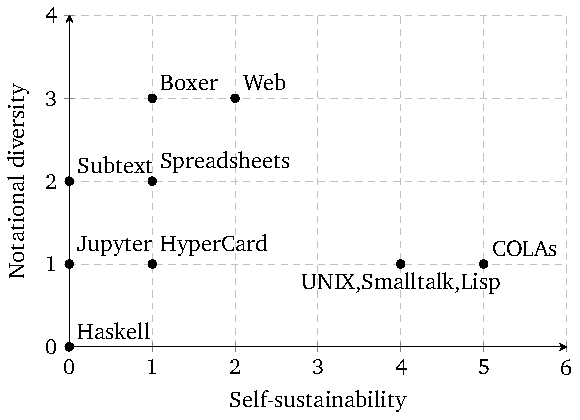
\includegraphics[width=0.6\linewidth]{plot-figure0.pdf}
  \caption{One 2-dimensional slice of the space of possible systems, to be examined in more detail in Section\ \ref{exploring-the-design-space}.\label{fig:tech-dims-diagram}}
\end{figure}

\hypertarget{related-work}{%
\section{Related work}\label{related-work}}

While we do have new ideas to propose, part of our contribution is
integrating a wide range of \emph{existing} concepts under a common
umbrella. This work is spread out across different domains, but each
part connects to programming systems or focuses on a specific
characteristic they may have.

\paragraph{From languages to systems.}

Our approach lies between a narrow focus on programming languages and a
broad focus on programming as a socio-political and cultural subject.
Our concept of a programming system is technical in scope, although we
acknowledge the technical side often has important social implications
as in the case of the ``Adoptability'' dimension
(Section~\ref{adoptability}). This contrasts with the more
socio-political focus found in Tchernavskij\DIFaddbegin \DIFadd{~}\DIFaddend \cite{TcherDiss} or in
software studies\DIFaddbegin \DIFadd{~}\DIFaddend \cite{SwStudies}. It overlaps with Kell's
conceptualization of UNIX, Smalltalk, and Operating Systems
generally~\cite{KellOS}, and we have ensured that UNIX has a place in
our framework.

The distinction between more narrow \emph{programming languages} and
broader \emph{programming systems} is more subtle. Richard Gabriel noted
an invisible paradigm shift from the study of ``systems'' to the study
of ``languages'' in computer science\DIFaddbegin \DIFadd{~}\DIFaddend \cite{PLrev}, and this observation
informs our distinction here. One consequence of the change is that a
\emph{language} is often formally specified apart from any specific
implementations, while \emph{systems} resist formal specification and
are often \emph{defined by} an implementation. We recognize programming
language implementations as a \emph{small region} of the space of
possible systems, at least as far as interaction and notations might go.
Hence we refer to the \emph{interactive programming system} aspects of
languages, such as text editing and command-line workflow.

\paragraph{Programming systems research.}

There is renewed interest in programming systems in \DIFdelbegin \DIFdel{both industry and
research, but the holistic programming systems view is more often
adopted in work on }\DIFdelend \DIFaddbegin \DIFadd{the form of recent
}\DIFaddend non-traditional programming tools:

\begin{itemize}
\tightlist
\item
  Computational notebooks such as Jupyter\DIFaddbegin \DIFadd{~\mbox{%DIFAUXCMD
\cite{Jupyter} }\hspace{0pt}%DIFAUXCMD
}\DIFaddend simplify data
  analysis by combining code snippets with text and visual output. They
  are backed by stateful ``kernels'' and used interactively.
\item
  ``Low code'' end-user programming systems allow application
  development (mostly) through a GUI. One example is
  Coda\DIFaddbegin \DIFadd{~}\DIFaddend \cite{CodaWeb}, which combines tables, formulas, and scripts to
  enable non-technical people to build ``applications as documents''.
\item
  Domain-specific programming systems such as Dark\DIFaddbegin \DIFadd{~\mbox{%DIFAUXCMD
\cite{DarkWeb}}\hspace{0pt}%DIFAUXCMD
}\DIFaddend , which
  claims a ``holistic'' programming experience for cloud API services.
  This includes a language, a direct manipulation editor, and
  near-instantaneous building and deployment.
\item
  Even for general purpose programming with conventional tools, systems
  like Replit\DIFaddbegin \DIFadd{~\mbox{%DIFAUXCMD
\cite{ReplitWeb} }\hspace{0pt}%DIFAUXCMD
}\DIFaddend have demonstrated the benefits of
  integrating all needed languages, tools, and user interfaces into a
  seamless experience, available from the browser, that requires no
  setup.
\end{itemize}

Research that follows the programming systems perspective can be found
in a number of research venues. Those include Human-Computer Interaction
conferences such as \href{https://uist.acm.org/}{UIST}\footnote{ACM
  Symposium on User Interface Software and Technology} and
\href{https://conferences.computer.org/VLHCC/}{VL/HCC}\footnote{IEEE
  Symposium on Visual Languages and Human-Centric Computing}. However,
work in those often emphasizes the user experience over technical
description. Programming systems are often presented in workshops such
as \href{https://liveprog.org/}{LIVE} and
\href{https://2021.programming-conference.org/home/px-2021}{PX}\footnote{Programming
  eXperience}. However, work in those venues is often limited to the
authors' individual perspectives and suffers from the aforementioned
difficulty of comparing to other systems.

Concrete examples of systems appear throughout the paper. Recent systems
which motivated some of our dimensions include Subtext\DIFaddbegin \DIFadd{~}\DIFaddend \cite{Subtext},
which combines code with its live execution in a single editable
representation; Sketch-n-sketch\DIFaddbegin \DIFadd{~}\DIFaddend \cite{SnS}, which can synthesize code by
direct manipulation of its outputs; Hazel\DIFaddbegin \DIFadd{~}\DIFaddend \cite{Hazel}, a live
functional programming environment with typed holes to enable execution
of incomplete or ill-typed programs; and Webstrates\DIFaddbegin \DIFadd{~}\DIFaddend \cite{Webstrates},
which extends Web pages with real-time sharing of state.

\paragraph{Already-known characteristics.}

There are several existing projects identifying characteristics of
programming systems. Some revolve around a single one, such as levels of
liveness\DIFaddbegin \DIFadd{~}\DIFaddend \cite{Liveness}, or plurality and
communicativity\DIFaddbegin \DIFadd{~}\DIFaddend \cite{KellComm}. Others propose an entire collection.
\emph{Memory Models of Programming Languages}~\cite{MemMod} identifies
the ``everything is an X'' metaphors underlying many programming
languages; the \emph{Design Principles of Smalltalk}~\cite{STdesign}
documents the philosophical goals and dicta used in the design of
Smalltalk; the ``Gang of Four'' \emph{Design Patterns}~\cite{DesPats}
catalogues specific implementation tactics; and the \emph{Cognitive
Dimensions of Notation}~\cite{CogDims} introduces a common vocabulary
for software's \emph{notational surface} and for identifying their
trade-offs.

The latter two directly influence our proposal. Firstly, the Cognitive
Dimensions are a set of qualitative properties which can be used to
analyze \emph{notations}. We wish to extend this approach to the
``rest'' of a system, beyond its notation, with \emph{Technical}
Dimensions. Secondly, our individual dimensions naturally fall under
larger \emph{clusters} that we present in a regular format, similar to
the presentation of the classic Design Patterns. As for characteristics
identified by others, part of our contribution is to integrate them
under a common umbrella: liveness, pluralism, and uniformity metaphors
(``everything is an X''), which have already been identified by others,
become dimensions in our framework.

\paragraph{Methodology.}

We follow the attitude of \emph{Evaluating Programming
Systems}~\cite{EvProgSys} in distinguishing our work from HCI methods
and empirical evaluation. We are generally concerned with
characteristics that are not obviously amenable to statistical analysis
(e.g.~mining software repositories) or experimental methods like
controlled user studies, so numerical quantities are generally not
featured.

Similar development seems to be taking place in HCI research focused on
user interfaces. The UIST guidelines\DIFaddbegin \DIFadd{~}\DIFaddend \cite{UISTAuthor} instruct authors
to evaluate system contributions holistically, and the community has
developed heuristics for such evaluation, such as \emph{Evaluating User
Interface Systems Research}~\cite{EvUISR}. Our set of dimensions offers
similar heuristics for identifying interesting aspects of programming
systems, though they focus more on underlying technical properties than
the surface interface.

Finally, we believe that the aforementioned paradigm shift from
programming systems to programming languages has hidden many ideas about
programming that are worthwhile recovering and developing
further\DIFaddbegin \DIFadd{~}\DIFaddend \cite{ComplementaryBasic}. Thus our approach is related to the
idea of \emph{complementary science} developed by Chang~\cite{Chang} in
the context of history and philosophy of science. Chang argues that even
in disciplines like physics, superseded or falsified theories may still
contain interesting ideas worth documenting. In the field of
programming, where past systems are discarded for many reasons besides
empirical failure, Chang's \emph{complementary science} approach seems
particularly suitable.

\paragraph{Programming systems deserve a theory too!}

In short, while there is a theory for programming languages, programming
\emph{systems} deserve a theory too. It should apply from the small
scale of language implementations to the vast scale of operating
systems. It should be possible to analyse the common and unique features
of different systems, to reveal new possibilities, and to build on past
work in an effective manner. In Kuhnian terms, it should enable a body
of ``normal science'': filling in the map of the space of possible
systems (Figure \ref{fig:tech-dims-diagram}), thereby forming a
knowledge repository for future designers.

\hypertarget{programming-systems}{%
\section{Programming systems}\label{programming-systems}}

We introduce the notion of a \emph{programming system} through a number
of \DIFdelbegin \DIFdel{examples, classified following the style of Lehman \mbox{%DIFAUXCMD
\cite{SPEPrograms}
}\hspace{0pt}%DIFAUXCMD
into three broad types. These are loosely inspired by the notions of
}\emph{\DIFdel{languages}}%DIFAUXCMD
\DIFdel{, }\emph{\DIFdel{operating systems}} %DIFAUXCMD
\DIFdel{and }\emph{\DIFdel{applications}}%DIFAUXCMD
\DIFdelend \DIFaddbegin \DIFadd{example systems. We draw them from three broad reference classes}\DIFaddend :

\begin{itemize}
\item
  \DIFdelbegin \textbf{\DIFdel{L-type programming systems}} %DIFAUXCMD
\DIFdel{are software }\DIFdelend \DIFaddbegin \DIFadd{Software }\DIFaddend ecosystems built around a text-based programming
  \emph{language}. They consist of a set of tools such as compilers,
  debuggers, and profilers. These tools may exist as separate
  command-line programs, or within an Integrated Development
  Environment.
\item
  \DIFdelbegin \textbf{\DIFdel{O-type programming systems}} %DIFAUXCMD
\DIFdel{resemble }\DIFdelend \DIFaddbegin \DIFadd{Those that resemble an }\DIFaddend \emph{operating \DIFdelbegin \DIFdel{systems}\DIFdelend \DIFaddbegin \DIFadd{system}\DIFaddend } \DIFaddbegin \DIFadd{(OS) }\DIFaddend in that they
  structure the execution environment and encompass the resources of an
  entire machine (physical or virtual). They provide a common interface
  for communication, both between the user and the computer, and between
  programs themselves.
\item
  \DIFdelbegin \textbf{\DIFdel{A-type programming systems}} %DIFAUXCMD
\DIFdel{are programmable
  }\DIFdelend \DIFaddbegin \DIFadd{Programmable }\DIFaddend \emph{applications}\DIFdelbegin \DIFdel{. They are }\DIFdelend \DIFaddbegin \DIFadd{, }\DIFaddend typically optimized for a specific
  domain, \DIFdelbegin \DIFdel{and offer }\DIFdelend \DIFaddbegin \DIFadd{offering }\DIFaddend a limited degree of programmability which may be
  increased with newer versions.
\end{itemize}

We will \DIFdelbegin \DIFdel{illustrate each of these types with several examples}\DIFdelend \DIFaddbegin \DIFadd{proceed to detail some systems under this grouping}\DIFaddend . This will
provide an intuition for the notion of a programming system and
establish a collection of go-to examples for the rest of the paper.

\DIFdelbegin %DIFDELCMD < \hypertarget{l-type-programming-systems}{%
%DIFDELCMD < \subsection{L-type programming
%DIFDELCMD < systems}\label{l-type-programming-systems}}
%DIFDELCMD < %%%
\DIFdelend \DIFaddbegin \hypertarget{systems-based-around-languages}{%
\subsection{Systems based around
languages}\label{systems-based-around-languages}}
\DIFaddend 

We see programming systems as (collections of) software artifacts that
make it possible to construct programs, debug them, and turn them into
operational, maintained, and evolvable artifacts running on an
appropriate hardware. Text-based programming languages sit within
programming systems whose boundaries are not explicitly defined. To
speak of a programming system, we need to consider a language with, at
minimum, an editor and a compiler or interpreter. However, the exact
boundaries are a design choice that significantly affects our analysis.

\paragraph{Java with the Eclipse ecosystem.}

Java\DIFaddbegin \DIFadd{~\mbox{%DIFAUXCMD
\cite{Java} }\hspace{0pt}%DIFAUXCMD
}\DIFaddend cannot be viewed as a programming system on its own,
but it is one if we consider it as embedded in an ecosystem of tools.
There are multiple ways to delineate this, resulting in different
analyses. A minimalistic programming system would consist of a text
editor to write Java code and a command line compiler. A more realistic
system is Java as embedded in the Eclipse IDE\DIFaddbegin \DIFadd{~\mbox{%DIFAUXCMD
\cite{Eclipse}}\hspace{0pt}%DIFAUXCMD
}\DIFaddend . The
programming systems view allows us to see all there is beyond the
textual code. In the case of Eclipse, this includes the debugger,
refactoring tools, testing and modelling tools, GUI designers, and so
on. This delineation yields a programming system that is powerful and
convenient, but has a large number of concepts and secondary notations.

\paragraph{Haskell tools ecosystem.}

Haskell is an even more language-focused programming system. It is used
through the command-line \emph{GHC} compiler\DIFaddbegin \DIFadd{~\mbox{%DIFAUXCMD
\cite{GHC} }\hspace{0pt}%DIFAUXCMD
}\DIFaddend and \emph{GHCi}
REPL, alongside a text editor that provides features like syntax
highlighting and auto-completion. In general, we can consider any editor
that supports the Language Server Protocol\DIFaddbegin \DIFadd{~}\DIFaddend \cite{LSP}.

Haskell is mathematically rooted and relies on mathematical intuition
for understanding many of its concepts. This background is also
reflected in the notations it uses. In addition to the concrete language
syntax for writing code, the ecosystem also uses an informal
mathematical notation for writing about Haskell (e.g.~in academic papers
or on the whiteboard). This provides an additional tool for manipulating
Haskell programs. Experiments on paper can provide a kind of rapid
feedback that other systems may provide through live programming.

\paragraph{From REPLs to notebooks.}

A different kind of developer ecosystem that evolved around a
programming language is the Jupyter notebook platform\DIFaddbegin \DIFadd{~\mbox{%DIFAUXCMD
\cite{Jupyter}}\hspace{0pt}%DIFAUXCMD
}\DIFaddend . In
Jupyter, data scientists write scripts divided into notebook cells,
execute them interactively and see the resulting data and visualizations
directly in the notebook itself. This brings together the REPL, which
dates back to conversational implementations of Lisp in the 1960s, with
literate programming\DIFaddbegin \DIFadd{~}\DIFaddend \cite{LiterateProg} used in the late 1980s in
Mathematica 1.0\DIFaddbegin \DIFadd{~\mbox{%DIFAUXCMD
\cite{Mathematica}}\hspace{0pt}%DIFAUXCMD
}\DIFaddend .

As a programming system, Jupyter has a number of interesting
characteristics. The primary outcome of programming is the notebook
itself, rather than a separate application to be compiled and run. The
code lives in a document format, interleaved with other notations. Code
is written in small parts that are executed quickly, offering the user
more rapid feedback than in conventional programming. A notebook can be
seen as a trace of how the result has been obtained, yet one often
problematic feature of notebooks is that some allow the user to run code
blocks out-of-order. The code manipulates mutable state that exists in a
``kernel'' running in the background. Thus, retracing one's steps in a
notebook is more subtle than in, say, Common Lisp\DIFaddbegin \DIFadd{~\mbox{%DIFAUXCMD
\cite{CommonLisp}}\hspace{0pt}%DIFAUXCMD
}\DIFaddend ,
where the \texttt{dribble} function would directly record the user's
session to a file.

\DIFdelbegin %DIFDELCMD < \hypertarget{o-type-programming-systems}{%
%DIFDELCMD < \subsection{O-type programming
%DIFDELCMD < systems}\label{o-type-programming-systems}}
%DIFDELCMD < %%%
\DIFdelend \DIFaddbegin \hypertarget{os-like-programming-systems}{%
\subsection{OS-like programming
systems}\label{os-like-programming-systems}}
\DIFaddend 

\DIFdelbegin \DIFdel{The first O-type programming systems emerged in }\DIFdelend \DIFaddbegin \DIFadd{These begin from }\DIFaddend the 1960s when it became possible to interact
one-on-one with a computer. First, time-sharing systems enabled
interactive shared use of a computer via a teletype; smaller computers
such as the PDP-1 and PDP-8 provided similar direct interaction, while
1970s workstations such as the Alto and Lisp Machines added graphical
displays and mouse input. \DIFaddbegin \DIFadd{These }\emph{\DIFadd{OS-like}} \DIFadd{systems stand out as
having the totalising scope of }\emph{\DIFadd{operating systems}}\DIFadd{, whether or not
they are }\emph{\DIFadd{officially}} \DIFadd{considered as such.
}\DIFaddend 

\paragraph{MacLisp and Interlisp.}

LISP 1.5\DIFaddbegin \DIFadd{~}\DIFaddend \cite{LISP15} arrived before the rise of interactive computers,
but the existence of an interpreter and the absence of declarations made
it natural to use Lisp interactively, with the first such
implementations appearing in the early 1960s. Two branches of the Lisp
family\DIFaddbegin \DIFadd{~}\DIFaddend \cite{LispEvolve}, MacLisp and the later Interlisp, embraced the
interactive ``conversational'' way of working, first through a teletype
and later using the screen and keyboard.

Both MacLisp and Interlisp adopted the idea of \emph{persistent address
space}. Both program code and program state were preserved when powering
off the system, and could be accessed and modified interactively as well
as programmatically using the \emph{same means}. Lisp Machines embraced
the idea that the machine runs continually and saves the state to disk
when needed. Today, this is widely seen in cloud-based services like
Google Docs and online IDEs. Another idea pioneered in MacLisp and
Interlisp was the use of \emph{structure editors}. These let programmers
work with Lisp data structures not as sequences of characters, but as
nested lists. In Interlisp, the programmer would use commands such as
\texttt{*P} to print the current expression, or \texttt{*(2\ (X\ Y))} to
replace its second element with the argument \texttt{(X\ Y)}. The PILOT
system\DIFaddbegin \DIFadd{~}\DIFaddend \cite{Pilot} offered even more sophisticated conversational
features. For typographical errors and other slips, it would offer an
automatic fix for the user to interactively accept, modifying the
program in memory and resuming execution.

\paragraph{Smalltalk.}

Smalltalk appeared in the 1970s with a distinct ambition of providing
``dynamic media which can be used by human beings of all
ages''\DIFaddbegin \DIFadd{~}\DIFaddend \cite{PersonalDynMedia}. The authors saw computers as
\emph{meta-media} that could become a range of other media for
education, discourse, creative arts, simulation and other applications
not yet invented. Smalltalk was designed for single-user workstations
with a graphical display, and pioneered this display not just for
applications but also for programming itself. In Smalltalk 72, one wrote
code in the bottom half of the screen using a structure editor
controlled by a mouse, and menus to edit definitions. In Smalltalk-76
and later, this had switched to text editing embedded in a \emph{class
browser} for navigating through classes and their methods.

Similarly to Lisp systems, Smalltalk adopts the persistent address space
model of programming where all objects remain in memory, but based on
\emph{objects} and \emph{message passing} rather than \emph{lists}. Any
changes made to the system state by programming or execution are
preserved when the computer is turned off. Lastly, the fact that much of
the Smalltalk environment is implemented in itself makes it possible to
extensively modify the system from within.

\paragraph{UNIX.}

We \DIFdelbegin \DIFdel{included }\DIFdelend \DIFaddbegin \DIFadd{include }\DIFaddend Lisp and Smalltalk in \DIFdelbegin \DIFdel{the O-type }\DIFdelend \DIFaddbegin \DIFadd{this group }\DIFaddend because they function as
operating systems in many ways. On specialized machines, like the Xerox
Alto and Lisp machines, the user started their machine directly in the
Lisp or Smalltalk environment and was able to do everything they needed
from \emph{within} the system. Nowadays, however, this experience is
associated with UNIX and its descendants on a vast range of commodity
machines.

UNIX illustrates the fact that many aspects of programming systems are
shaped by their intended target audience. Built for computer
hackers\DIFaddbegin \DIFadd{~\mbox{%DIFAUXCMD
\cite{Hackers}}\hspace{0pt}%DIFAUXCMD
}\DIFaddend , its abstractions and interface are close to the
machine. Although historically linked to the C language, UNIX developed
a language-agnostic set of abstractions that make it possible to use
multiple programming languages in a single system. While everything is
an object in Smalltalk, the ontology of the UNIX system consists of
files, memory, executable programs, and running processes. Note the
explicit ``stage'' distinction here: UNIX distinguishes between volatile
\emph{memory} structures, which are lost when the system is shut down,
and non-volatile \emph{disk} structures that are preserved. This
distinction between types of memory is considered, by Lisp and
Smalltalk, to be an implementation detail to be abstracted over by their
persistent address space. Still, this did not prevent the UNIX ontology
from supporting a pluralistic ecosystem of different languages and
tools.

\paragraph{Early and late Web.}

The Web evolved\DIFaddbegin \DIFadd{~\mbox{%DIFAUXCMD
\cite{DotCom} }\hspace{0pt}%DIFAUXCMD
}\DIFaddend from a system for sharing and organizing
information to a \emph{programming system}. Today, it consists of a wide
range of server-side programming tools, JavaScript and languages that
compile to it, and notations like HTML and CSS. As a programming system,
the ``modern 2020s web'' is reasonably distinct from the ``early 1990s
web''. In the early web, JavaScript code was distributed in a form that
made it easy to copy and re-use existing scripts, which led to
enthusiastic adoption by non-experts---recalling the birth of
microcomputers like Commodore 64 with BASIC a decade earlier.

In the ``modern web'', multiple programming languages treat JavaScript
as a compilation target, and JavaScript is also used as a language on
the server-side. This web is no longer simple enough to encourage
copy-and-paste remixing of code from different sites. However, it does
come with advanced developer tools that provide functionality resembling
early interactive programming systems like Lisp and Smalltalk. The
\emph{Document Object Model (DOM)} structure created by a web page is
transparent, accessible to the user and modifiable through the built-in
browser inspector tools. Third-party code to modify the DOM can be
injected via extensions. The DOM almost resembles the tree/graph model
of Smalltalk and Lisp images, lacking the key persistence property. This
limitation, however, is being addressed by Webstrates~\cite{Webstrates}.

\DIFdelbegin %DIFDELCMD < \hypertarget{a-type-programming-systems}{%
%DIFDELCMD < \subsection{A-type programming
%DIFDELCMD < systems}\label{a-type-programming-systems}}
%DIFDELCMD < %%%
\DIFdelend \DIFaddbegin \hypertarget{application-focused-systems}{%
\subsection{Application-focused
systems}\label{application-focused-systems}}
\DIFaddend 

The previously discussed programming systems were either universal, not
focusing on any particular kind of application, or targeted at broad
fields, such as Artificial Intelligence and symbolic data manipulation
in Lisp's case. In contrast, the \DIFdelbegin \DIFdel{A-type programming systems }\DIFdelend \DIFaddbegin \DIFadd{following examples }\DIFaddend focus on more narrow
kinds of applications that need to be built. Many support programming
based on rich interactions with specialized visual and textual
notations.

\paragraph{Spreadsheets.}

The first \DIFdelbegin \DIFdel{system, VisiCalc, }\DIFdelend \DIFaddbegin \DIFadd{spreadsheets }\DIFaddend became available in 1979 \DIFaddbegin \DIFadd{in
VisiCalc~\mbox{%DIFAUXCMD
\cite{VisiCalc, VisiCalc2} }\hspace{0pt}%DIFAUXCMD
}\DIFaddend and helped analysts perform budget
calculations. As programming systems, spreadsheets are notable for their
programming substrate (a two-dimensional grid) and evaluation model
(automatic re-evaluation). The programmability of spreadsheets developed
over time, acquiring features that made them into powerful programming
systems in a way VisiCalc was not. The final step was the 1993 inclusion
of \emph{macros} in Excel, later further extended with \emph{Visual
Basic for Applications}.

\DIFaddbegin \paragraph{\DIFadd{Graphical "languages".}}

\DIFadd{Efforts to support programming without relying on textual code can only
be called ``languages'' in a metaphorical sense. In these programming
systems, programs are made out of graphical structures as in
LabView~\mbox{%DIFAUXCMD
\cite{LabView} }\hspace{0pt}%DIFAUXCMD
or Programming-By-Example~\mbox{%DIFAUXCMD
\cite{PBE}}\hspace{0pt}%DIFAUXCMD
.
}

\DIFaddend \paragraph{HyperCard.}

While spreadsheets were designed to solve problems in a specific
application area, HyperCard\DIFaddbegin \DIFadd{~}\DIFaddend \cite{HyperCard} was designed around a
particular application format. Programs are ``stacks of cards''
containing multimedia components and controls such as buttons. These
controls can be programmed with pre-defined operations like ``navigate
to another card'', or via the HyperTalk scripting language for anything
more sophisticated.

As a programming system, HyperCard is interesting for a couple of
reasons. It effectively combines visual and textual notation. Programs
appear the same way during editing as they do during execution. Most
notably, HyperCard supports gradual progression from the ``user'' role
to ``developer'': a user may first use stacks, then go on to edit the
visual aspects or choose pre-defined logic until, eventually, they learn
to program in HyperTalk.

\DIFdelbegin %DIFDELCMD < \hypertarget{technical-dimensions}{%
%DIFDELCMD < \section{Technical dimensions}\label{technical-dimensions}}
%DIFDELCMD < %%%
\DIFdelend \DIFaddbegin 
\includepdf[pages={2}]{table.pdf}
\DIFaddend 

\DIFdelbegin \DIFdel{We }\DIFdelend \DIFaddbegin \hypertarget{technical-dimensions-catalogue}{%
\section{Technical dimensions
catalogue}\label{technical-dimensions-catalogue}}

\DIFadd{Here, we }\DIFaddend present our proposed technical dimensions \DIFaddbegin \DIFadd{in great detail.
Please note that our intention is to provide a }\emph{\DIFadd{reference}} \DIFadd{to be
looked up and }\emph{\DIFadd{used}} \DIFadd{as needed, not something that should be read
from start to finish. Therefore, we recommend skimming through this for
anything particularly interesting before proceeding to
Section~\ref{evaluation}. There, we will reference several dimensions in
the context of a specific example, at which point it may be helpful to
come back for more detail. For a quick overview, we included a concise
reference sheet on the previous page, though it may make more sense
after reading the relevant sections.
}

\DIFadd{We present the dimensions }\DIFaddend grouped under \emph{clusters}. \DIFdelbegin \DIFdel{The clusters }\DIFdelend \DIFaddbegin \DIFadd{These }\DIFaddend may be
regarded as ``topics of interest'' or ``areas of inquiry'' when studying
a given system, grouping together related dimensions against which to
measure it.
\DIFdelbegin \DIFdel{We also include a
concise reference sheet on the next page, though it will make more sense
after reading the relevant sections.
}\DIFdelend 

Each cluster is named and opens with a boxed \emph{summary}, followed by
a longer \emph{discussion}, and closes with a list of any
\emph{relations} to other clusters along with any \emph{references} if
applicable. Within the main discussion, individual \emph{dimensions} are
listed. Sometimes, a particular value along a dimension (or a
combination of values along several dimensions) can be recognized as a
familiar pattern---perhaps with a name already established in the
literature. These are marked as \emph{examples}. Finally, interspersed
discussion that is neither a \emph{dimension} nor an \emph{example} is
introduced as a \emph{remark}.

\DIFdelbegin \DIFdel{For space reasons, we are only able to include one cluster,
}\emph{\DIFdel{customizability}}%DIFAUXCMD
\DIFdel{, in the main body of this paper. We encourage the
reader to peruse Appendix~\ref{dimensions-catalogue} for the full extent
of our proposed dimensions.
}\DIFdelend \DIFaddbegin \textbf{\DIFadd{NB: Kept the dimension catalogue in the appendix, as otherwise the diff is useless past this point. E.g. it just shows all of Section\ 5 in blue.}}
\DIFaddend 

\DIFdelbegin %DIFDELCMD < \hypertarget{discussion}{%
%DIFDELCMD < \section{Discussion}\label{discussion}}
%DIFDELCMD < %%%
\DIFdelend \DIFaddbegin \hypertarget{evaluation}{%
\section{Evaluation}\label{evaluation}}
\DIFaddend 

The technical dimensions \DIFdelbegin \DIFdel{framework is intended to assist designers of }\DIFdelend \DIFaddbegin \DIFadd{should be evaluated on the basis of how useful
they are for designing and analysing }\DIFaddend programming systems. \DIFdelbegin \DIFdel{This section illustrates two ways in which it can
be used}\DIFdelend \DIFaddbegin \DIFadd{To that end,
this section demonstrates two uses of the framework}\DIFaddend . First, we use the
dimensions to analyze the recent programming system Dark~\cite{DarkWeb},
explaining how it relates to past work and how it contributes to the
state of the art. Second, we use technical dimensions to identify a new
unexplored point in the design space of programming systems and envision
a new design that could emerge from the analysis.

\DIFdelbegin %DIFDELCMD < \hypertarget{evaluating-programming-systems}{%
%DIFDELCMD < \subsection{Evaluating programming
%DIFDELCMD < systems}\label{evaluating-programming-systems}}
%DIFDELCMD < %%%
\DIFdelend \DIFaddbegin \hypertarget{evaluating-the-dark-programming-system}{%
\subsection{Evaluating the Dark programming
system}\label{evaluating-the-dark-programming-system}}
\DIFaddend 

Dark is a programming system for building ``serverless backends'',
i.e.~services that are used by web and mobile applications. It aims to
make building such services easier by ``removing accidental
complexity''\footnote{https://roadmap.darklang.com/goals-of-dark-v2.html}
resulting from the large number of systems typically involved in their
deployment and operation. This includes infrastructure for
orchestration, scaling, logging, monitoring and versioning. Dark
provides integrated tooling (Figure~\ref{fig:dark}) for development and
is described as \emph{deployless}, meaning that deploying code to
production is instantaneous.

\begin{figure}
  \centering
  \DIFdelbeginFL %DIFDELCMD < 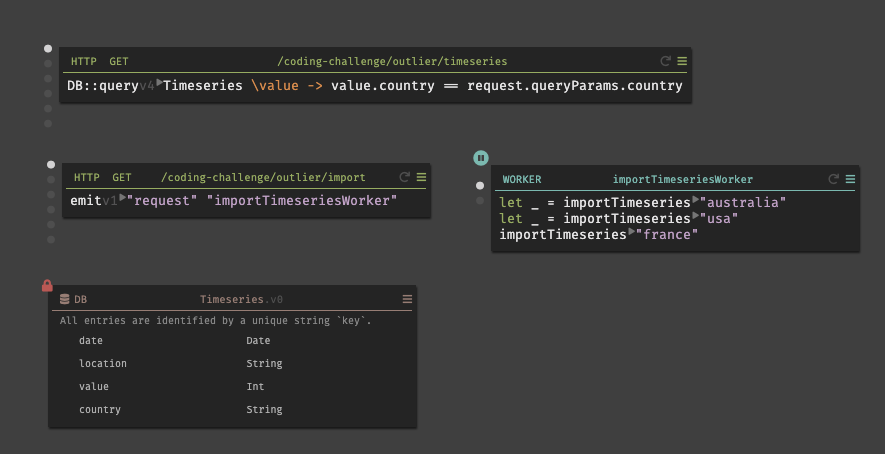
\includegraphics[width=1\linewidth]{dark.png}
%DIFDELCMD <   %%%
\DIFdelendFL \DIFaddbeginFL 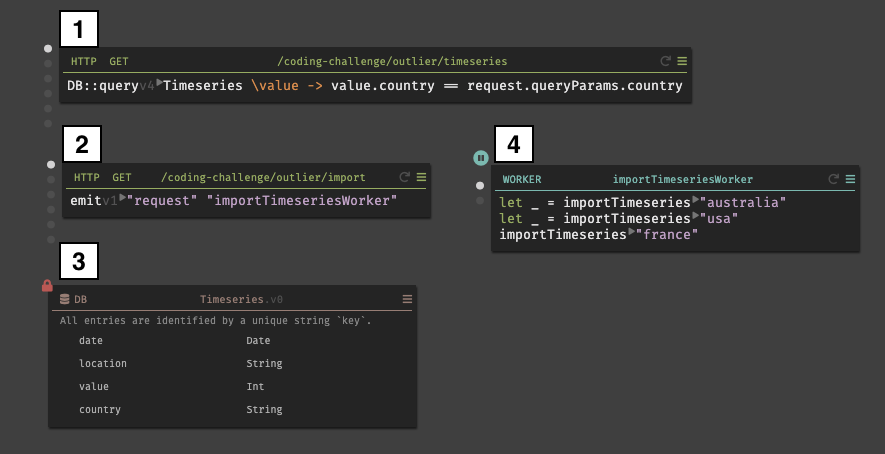
\includegraphics[width=1\linewidth]{dark-annotated.png}
  \DIFaddendFL \caption{\DIFdelbeginFL \DIFdelFL{The Dark programming environment showing a }\DIFdelendFL \DIFaddbeginFL \DIFaddFL{A }\DIFaddendFL simple web service \DIFdelbeginFL \DIFdelFL{comprising a database, }\DIFdelendFL \DIFaddbeginFL \DIFaddFL{in Dark consisting of }\DIFaddendFL two HTTP endpoints \DIFaddbeginFL \DIFaddFL{(1, 2), a database (3), }\DIFaddendFL and a worker \DIFaddbeginFL \DIFaddFL{(4)}\DIFaddendFL .\label{fig:dark}}
  \note{FROM https://medium.com/@wilk/dark-lang-an-uncommon-step-towards-the-future-of-programming-921cf7f38baf}
\end{figure}

Dark illustrates the need for the broader perspective of programming
systems. Of course, it contains a programming language, which is
inspired by OCaml and F\#. But Dark's distinguishing feature is that it
eliminates the many secondary systems needed for deployment of modern
cloud-based services. Those exist outside of a typical programming
language, yet form a major part of the complexity of the overall
development process.

With technical dimensions, we can go beyond the ``sales pitch'', look
behind the scenes, and better understand the interesting technical
aspects of Dark as a programming system. \DIFaddbegin \DIFadd{Table~\ref{tab:dark} summarises
the more detailed analysis that follows.
}\DIFaddend 

\DIFaddbegin \newcommand{\wrap}[1]{\parbox[t]{10cm}{#1}}
\renewcommand{\arraystretch}{1.3}

\begin{table}
\centering
\caption{\DIFaddFL{Summary of where Dark lies on some of the dimensions.}}
\begin{tabular}{ >{\raggedleft\arraybackslash}p{4.6cm} l }
\hline
\DIFaddFL{Dimension (CLUSTER) }& \DIFaddFL{Summary }\\ 
\hline\hline
\DIFaddFL{INTERACTION }\\
\DIFaddFL{Modes of Interaction }& 
\parbox[t]{10cm}{\DIFaddFL{Single integrated mode comprises development, debugging and operation ("deployless")}} \\
\DIFaddFL{Feedback Loops }& \parbox[t]{10cm}{\DIFaddFL{Code editing is triggered either by user or by unsupported HTTP request and changes are deployed automatically, allowing for }\emph{\DIFaddFL{immediate feedback}}}\\
\hline
\DIFaddFL{ERRORS  }\\
\DIFaddFL{Error Response }& \parbox[t]{10cm}{\DIFaddFL{When an unsupported HTTP request is received, programmer can write handler code using data from the request in the process}}\\
\hline
\DIFaddFL{CONCEPTUAL STRUCTURE    }\\
\DIFaddFL{Conceptual Integrity vs. Openness }& \parbox[t]{10cm}{\DIFaddFL{Abstractions at the domain specific high-level and the functional low-level are both carefully designed for conceptual integrity.}}\\
\DIFaddFL{Composability }& \parbox[t]{10cm}{
\DIFaddFL{User applications are composed from high-level primitives; the low-level uses composable functional abstractions (records, pipelines).}}\\
\DIFaddFL{Convenience }& \parbox[t]{10cm}{\DIFaddFL{Powerful high-level domain-specific abstractions are provided (HTTP, database, workers); core functional libraries exist for the low-level.}} \\
\hline
\DIFaddFL{ADOPTABILITY }\\
\DIFaddFL{Learnability }& \parbox[t]{10cm}{\DIFaddFL{High-level concepts will be immediately familiar to the target audience; low-level language has the usual learning curve of basic functional programming}}\\
\hline
\DIFaddFL{NOTATION    }\\
\DIFaddFL{Notational Structure }& \parbox[t]{10cm}{\DIFaddFL{Graphical notation for high-level concepts is complemented by structure editor for low-level code}} \\
\DIFaddFL{Uniformity }& \parbox[t]{10cm}{\DIFaddFL{Common notational structures are used for database and code, enabling the same editing construct for sequential structures (records, pipelines, tables)}}\\
\hline
\DIFaddFL{COMPLEXITY  }\\
\DIFaddFL{Factoring of Complexity }& \parbox[t]{10cm}{\DIFaddFL{Cloud infrastructure (deployment, orchestration, etc.) is provided by the Dark platform that is invisible to the programmer, but also cannot be modified}}\\
\DIFaddFL{Level of Automation }& \parbox[t]{10cm}{\DIFaddFL{Current implementation provides basic infrastructure, but a higher degree of automation in the platform can be provided in the future, e.g. for scalability}} \\
\hline
\DIFaddFL{CUSTOMIZABILITY}\\   
\DIFaddFL{Staging of Customization }& \parbox[t]{10cm}{\DIFaddFL{System can be modified while running and changes are persisted, but they have to be made in the Dark editor, which is distinct from the running service}}
\end{tabular}
\label{tab:dark}
\end{table}

\DIFaddend \hypertarget{dimensional-analysis-of-dark}{%
\subsubsection{Dimensional analysis of
Dark}\label{dimensional-analysis-of-dark}}

\paragraph{Modes of interaction and feedback loops.}

Conventional \emph{modes of interaction}
(\ref{dimension-modes-of-interaction}) include running, editing and
debugging. For modern web services, running refers to operation in a
cloud-based environment that typically comes with further kinds of
feedback (logging and monitoring). The key design decision of Dark is to
integrate all these different modes of interaction into a single one.
This tight integration allows Dark to provide a more immediate
\emph{feedback loop} (\ref{dimension-feedback-loops}) where code changes
become immediately available not just to the developer, but also to
external users. The integrated mode of interaction is reminiscent of the
image-based environment in Smalltalk; Dark advances the state of art by
using this model in a multi-user, cloud-based context.

\paragraph{Feedback loops and error response.}

The integration of development and operation also makes it possible to
use \emph{errors} occurring during operation to drive development.
Specifically, when a Dark service receives a request that is not
supported, the user can build a handler\DIFaddbegin \DIFadd{~\mbox{%DIFAUXCMD
\cite{DarkErrors} }\hspace{0pt}%DIFAUXCMD
}\DIFaddend to provide a
response---taking advantage of the live data that was sent as part of
the request. In terms of our dimensions, this is a kind of \emph{error
response} (\ref{dimension-error-response}) that was pioneered by the
PILOT system for Lisp~\cite{Pilot}. Dark does this not just to respond
to errors, but also as the primary development mechanism, which we might
call \emph{Error-Driven Development.} This way, Dark users can construct
programs with respect to sample input values.

\paragraph{Conceptual structure and learnability.}

Dark programs are expressed using high-level concepts that are specific
to the domain of server-side web programming: HTTP request handlers,
databases, workers and scheduled jobs. These are designed to reduce
accidental complexity and aim for high \emph{conceptual integrity}
(\ref{dimension-conceptual-integrity-vs.-openness}). At the level of
code, Dark uses a general-purpose functional language that emphasizes
certain concepts, especially records and pipelines. The high-level
concepts contribute to \emph{learnability}
(\ref{dimension-learnability}) of the system, because they are highly
domain-specific and will already be familiar to its intended users.

\paragraph{Notational structure and uniformity.}

Dark uses a combination of graphical editor and code. The two aspects of
the notation follow the \emph{complementing notations}
(\ref{dimension-notational-structure}) pattern. The windowed interface
is used to work with the high-level concepts and code is used for
working with low-level concepts. At the high level, code is structured
in freely positionable boxes on a 2D surface. Unlike Boxer\DIFaddbegin \DIFadd{~}\DIFaddend \cite{Boxer},
these boxes do not nest and the space cannot be used for other content
(say, for comments, architectural illustrations or other media). Code at
the low level is manipulated using a syntax-aware structure editor,
showing inferred types and computed live values for pure functions. It
also provides special editing support for records and pipelines,
allowing users to add fields and steps respectively.

\paragraph{Factoring of complexity and automation.}

One of the advertised goals of Dark is to remove accidental complexity.
This is achieved by collapsing the heterogeneous stack of technologies
that are typically required for development, cloud deployment,
orchestration and operation. Dark hides this via \emph{factoring of
complexity} (\ref{dimension-factoring-of-complexity}). The advanced
infrastructure is provided by the Dark platform and is hidden from the
user. The infrastructure is programmed explicitly and there is no need
for sophisticated automation (\ref{dimension-level-of-automation}). This
factoring of functionality that was previously coded manually follows a
similar pattern as the development of garbage collection in high-level
programming languages.

\paragraph{Customizability.}

The Dark platform makes a clear distinction between the platform itself
and the user application, so \emph{self-sustainability}
(\ref{dimension-self-sustainability}) is not an objective. The strict
division between the platform and user (related to its aforementioned
\emph{factoring of complexity}) means that changes to Dark require
modifying the platform source code itself, which is available under a
license that solely allows using it for the purpose of contributing.
Similarly, applications themselves are developed by modifying and adding
code, requiring destructive access to it---so \emph{additive authoring}
(\ref{dimension-addressing-and-externalizability}) is not exhibited at
either level. Thanks to the integration of execution and development,
persistent changes may be made during execution (c.f. \emph{staging of
customization}, \ref{dimension-staging-of-customization}) but this is
done through the Dark editor, which is separate from the running
service.

\hypertarget{technical-innovations-of-dark}{%
\subsubsection{Technical innovations of
Dark}\label{technical-innovations-of-dark}}

This analysis reveals a number of interesting aspects of the Dark
programming system. The first is the tight integration of different
\emph{modes of interaction} which collapses a heterogeneous stack of
technologies, makes Dark \emph{learnable}, and allows quick feedback
from deployed services. The second is the use of \emph{error response}
to guide the development of HTTP handlers. Thanks to the technical
dimensions framework, each of these can be more precisely described. It
is also possible to see how they may be supported in other programming
systems. The framework also points to possible alternatives (and perhaps
improvements) such as building a more self-sustainable system that has
similar characteristics to Dark, but allows greater flexibility in
modifying the platform from within itself.

\hypertarget{exploring-the-design-space}{%
\subsection{Exploring the design
space}\label{exploring-the-design-space}}

With a little work, technical dimensions can let us see patterns or gaps
in the design space by plotting their values on a simple scatterplot.
Here, we will look at two dimensions, \emph{notational
diversity}\footnote{This is simply the dimension we named as
  \emph{uniformity of notations}
  (\ref{dimension-uniformity-of-notations}), but flipped in the opposite
  direction.} and \emph{self-sustainability}, for the following
programming systems: Haskell, Jupyter notebooks, Boxer, HyperCard, the
Web, spreadsheets, Lisp, Smalltalk, UNIX, and COLAs.

While our choice to \DIFdelbegin \DIFdel{identify and }\DIFdelend describe dimensions as qualitative concepts was
necessary for coming up with them, \emph{some} way of generating numbers
is clearly necessary for visualizing their relationships like this. For
simplicity,\footnote{There are undoubtedly many ways to turn our
  descriptions into various measures, with strengths and weaknesses for
  different purposes, but this is beyond the scope of the present paper.
  Here, we merely wish to demonstrate that such a thing is possible and
  show what one can do with the results.} we adopt the following scheme.
For each dimension, we distill the main idea into several yes/no
questions (Appendix~\ref{making-dimensions-quantitative}) that capture
enough of the distinctions we observe between the systems we wish to
plot. Then, for each system, we add up the number of ``yes'' answers and
obtain a plausible score for the dimension.

\begin{figure}
  \centering
  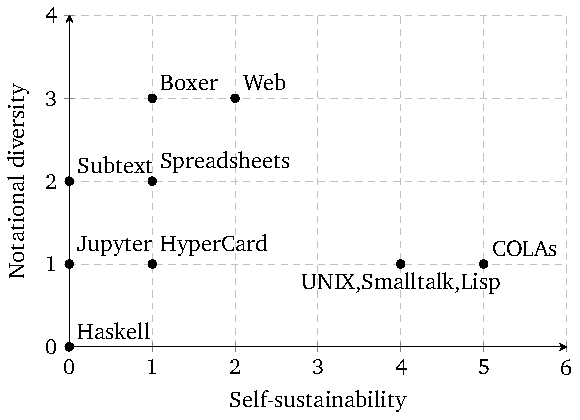
\includegraphics[width=0.6\linewidth]{plot-figure0.pdf}
  \caption{Example programming systems (or system families) measured against \emph{self-sustainability} and \emph{notational diversity}, revealing an absence of systems with a high degree of both. \label{fig:design-space-plot}}
\end{figure}

Figure~\ref{fig:design-space-plot} shows the results we obtained with
our sets of questions. It shows that \DIFdelbegin \DIFdel{the A-types }\DIFdelend \DIFaddbegin \DIFadd{application-focused systems }\DIFaddend span a
range of notational diversity, but only within fairly low
self-sustainability. The \DIFdelbegin \DIFdel{O-types }\DIFdelend \DIFaddbegin \DIFadd{``OS-likes'' (Section
\ref{os-like-programming-systems}) }\DIFaddend cluster in an ``island'' at the
right, sharing identical notational diversity and near-identical
self-sustainability. There is also a conspicuous blank space at the
top-right, representing an unexplored combination of high values on both
dimensions. With other pairs of dimensions, we might take this as
evidence of an oppositional relationship, such that more of one
inherently means less of the other (perhaps looking for a single new
dimension that describes this better.) In this case, though, there is no
obvious conflict between having many notations and being able to change
a system from within. Therefore, we interpret the gap as a new
opportunity to try out: combine the self-sustainability of COLAs with
the notational diversity of Boxer and Web development. In fact, this is
more or less the forthcoming dissertation of the primary author.

\hypertarget{conclusions}{%
\section{Conclusions}\label{conclusions}}

There is a renewed interest in developing new programming systems. Such
systems go beyond the simple model of code written in a programming
language using a more or less sophisticated text editor. They combine
textual and visual notations, create programs through rich graphical
interactions, and challenge accepted assumptions about program editing,
execution and debugging. Despite the growing number of novel programming
systems, it remains difficult to evaluate the design of programming
systems and see how they improve over work done in the past. To address
the issue, we proposed a framework of ``technical dimensions'' that
captures essential characteristics of programming systems in a
qualitative but rigorous way.

The framework of technical dimensions puts the vast variety of
programming systems, past and present, on a common footing of
commensurability. This is crucial to enable the strengths of each to be
identified and, if possible, combined by designers of the next
generation of programming systems. As more and more systems are assessed
in the framework, a picture of the space of possibilities will gradually
emerge. Some regions will be conspicuously empty, indicating unrealized
possibilities that could be worth trying. In this way, a domain of
``normal science'' is created for the design of programming systems.

\acks

(To be completed for publication.)

\appendix
\DIFaddbegin 

\DIFaddend \newpage

\hypertarget{making-dimensions-quantitative}{%
\section{Making dimensions
quantitative}\label{making-dimensions-quantitative}}

To generate numerical co-ordinates for \emph{self-sustainability} and
\emph{notational diversity}, we split both dimensions into a small
number of yes/no questions and counted the ``yes'' answers for each
system. We came up with the questions informally, with the goal of
achieving three things:

\begin{enumerate}
\def\labelenumi{\arabic{enumi}.}
\tightlist
\item
  To capture the basic ideas or features of the dimension
\item
  To make prior impressions more precise (i.e.~to roughly match where we
  intuitively felt certain key systems fit, but provide precision and
  possible surprises for systems we were not as confident about.)
\item
  To be the fewest in number necessary to attain the above
\end{enumerate}

The results of this process were as follows, along with a brief
rationale for each question. Afterwards, we will close with some
remarks.

\newcommand{\y}{\ding{52}}
\newcommand{\n}{}

\hypertarget{self-sustainability}{%
\subsection{Self-sustainability}\label{self-sustainability}}

Questions:

\begin{enumerate}
\def\labelenumi{\arabic{enumi}.}
\tightlist
\item
  \emph{Can you add new items to system namespaces without a restart?}
  The canonical example of this is in JavaScript, where ``built-in''
  classes like \texttt{Array} or \texttt{Object} can be augmented at
  will (and destructively modified, but that would be a separate point).
  Concretely, if a user wishes to make a new \texttt{sum} operation
  available to all Arrays, they are not \emph{prevented} from
  straightforwardly adding the method to the Array prototype as if it
  were just an ordinary object (which it is). Having to re-compile or
  even restart the system would mean that this cannot be meaningfully
  achieved from within the system. Conversely, being able to do this
  means that even ``built-in'' namespaces are modifiable by ordinary
  programs, which indicates less of a implementation level vs.~user
  level divide and seems important for self-sustainability.
\item
  \emph{Can programs generate programs and execute them?} This property,
  related to ``code as data'' or the presence of an \texttt{eval()}
  function, is a key requirement of self-sustainability. Otherwise,
  re-programming the system, beyond selecting from a predefined list of
  behaviors, will require editing an external representation and
  restarting it. If users can type text inside the system then they will
  be able to write code---yet this code will be inert unless the system
  can interpret internal data structures as programs and actually
  execute them.
\item
  \emph{Are changes persistent enough to encourage indefinite
  evolution?} If initial tinkering or later progress can be reset by
  accidentally closing a window, or preserved only through a convoluted
  process, then this discourages any long-term improvement of a system
  from within. For example, when developing a JavaScript application
  with web browser developer tools, it is possible to run arbitrary
  JavaScript in the console, yet these changes apply only to the running
  instance. After tinkering in the console with the advantage of
  concrete system state, one must still go back to the source code file
  and make the corresponding changes manually. When the page is
  refreshed to load the updated code, it starts from a fresh initial
  state. This means it is not worth using the \emph{running} system for
  any programming beyond tinkering.
\item
  \emph{Can you reprogram low-level infrastructure within the running
  system?} This is a hopefully faithful summary of how the COLAs work
  aims to go beyond Lisp and Smalltalk in this dimension.
\item
  \emph{Can the user interface be arbitrarily changed from within the
  system?} Whether classed as ``low-level infrastructure'' or not, the
  visual and interactive aspects of a system are a significant part of
  it. As such, they need to be as open to re-programming as any other
  part of it to classify as truly self-sustainable.
\end{enumerate}

\begin{tabular}{ c  c c c  c c c c  c c c c }
Question & \rot{Haskell}      & \rot{Jupyter} & \rot{HyperCard} & \rot{Subtext}
         & \rot{Spreadsheets} & \rot{Boxer}   & \rot{Web}       & \rot{UNIX}
         & \rot{Smalltalk}    & \rot{Lisp}    & \rot{COLAs} \\
\hline
1 & & & & & & & \ding{52}& \ding{52}& \ding{52}& \ding{52}& \ding{52}\\
2 & & & & & & & \ding{52}& \ding{52}& \ding{52}& \ding{52}& \ding{52}\\
3 & & & \ding{52}& & \ding{52}& \ding{52}& & \ding{52}& \ding{52}& \ding{52}& \ding{52}\\
4 & & & & & & & & & & & \ding{52}\\
5 & & & & & & & & \ding{52}& \ding{52}& \ding{52}& \ding{52}\\
\hline
Total & 0 & 0 & 1 & 0 & 1 & 1 & 2 & 4 & 4 & 4 & 5 \\
\end{tabular}

\hypertarget{notational-diversity}{%
\subsection{Notational diversity}\label{notational-diversity}}

Questions:

\begin{enumerate}
\def\labelenumi{\arabic{enumi}.}
\tightlist
\item
  \emph{Are there multiple syntaxes for textual notation?} Obviously,
  having more than one textual notation should count for notational
  diversity. However, for this dimension we want to take into account
  notations beyond the strictly textual, so we do not want this to be
  the only relevant question. Ideally, things should be weighted so that
  having a wide diversity of notations within some \emph{narrow class}
  is not mistaken for notational diversity in a more global sense. We
  want to reflect that UNIX, with its vast array of different languages
  for different situations, can never be as notationally diverse as a
  system with many languages \emph{and} many graphical notations, for
  example.
\item
  \emph{Does the system make use of GUI elements?} This is a focused
  class of non-textual notations that many of our example systems
  exhibit.
\item
  \emph{Is it possible to view and edit data as tree structures?} Tree
  structures are extremely common in programming, but they are usually
  worked with as text in some way. A few of our examples provide a
  graphical notation for this common data structure, so this is one way
  they can be differentiated from the rest.
\item
  \emph{Does the system allow freeform arrangement and sizing of data
  items?} We still felt Boxer and spreadsheets exhibited something not
  covered by the previous three questions, which is this. Within their
  respective constraints of rendering trees as nested boxes and
  single-level grids, they both provide for notational variation that
  can be useful to the user's context. These systems \emph{could} have
  decided to keep boxes neatly placed or cells all the same size, but
  the fact that they allow these to vary scores an additional point for
  notational diversity.
\end{enumerate}

\begin{tabular}{ c  c c c  c c c c  c c c c }
Question & \rot{Haskell}      & \rot{Jupyter} & \rot{HyperCard} & \rot{Subtext}
         & \rot{Spreadsheets} & \rot{Boxer}   & \rot{Web}       & \rot{UNIX}
         & \rot{Smalltalk}    & \rot{Lisp}    & \rot{COLAs} \\
\hline
1 & & & & & & & \ding{52}& \ding{52}& & & \ding{52}\\
2 & & \ding{52}& \ding{52}& \ding{52}& \ding{52}& \ding{52}& \ding{52}& & \ding{52}& & \\
3 & & & & \ding{52}& & \ding{52}& \ding{52}& & & \ding{52}& \\
4 & & & & & \ding{52}& \ding{52}& & & & & \\
\hline
Total & 0 & 1 & 1 & 2 & 2 & 3 & 3 & 1 & 1 & 1 & 1 \\
\end{tabular}

\hypertarget{remarks-and-future-work}{%
\subsection{Remarks and future work}\label{remarks-and-future-work}}

This task of quantifying dimensions forced us to drill down and decide
on more crisp definitions of what they should be. We recommend it as a
useful exercise even in the absence of a goal like generating a graph.

It is worth clarifying the meaning of what we have done here. It must
not be overlooked that this settling down on one particular definition
does not replace or obsolete the general qualitative descriptions of the
dimensions that we start with. Clearly, there are far too many sources
of variation in our process to consider our results here as final,
objective, the single correct definition of these dimensions, or
anything in this vein. Each of these sources of variation suggests
future work for interested parties:

\paragraph{Quantification goals.}

We sought numbers to generate a graph that roughly matched our own
intuitive placement of several example systems. In other words, we were
trying to make those intuitions more precise along with the dimensions
themselves. An entirely different approach would be to have no
``anchor'' at all, and to take whatever answers a given definition
produces as ground truth. However, this would demand more detail for
answering questions and generating them in the first place.

\paragraph{Question generation.}

We generated our questions informally and stopped when it seemed like
there were enough to make the important distinctions between example
points. There is huge room for variation here, though it seems
particularly hard to generate questions in any rigorous manner. Perhaps
we could take our \emph{self-sustainability} questions to be drawn from
a large set of ``actions you can perform while the system is running'',
which could be parametrized more easily. Similarly, our \emph{notational
diversity} questions tried to take into account a few classes of
notations---a more sophisticated approach might be to just count the
notations in a wide range of classes.

\paragraph{Answering the questions.}

We answered our questions by coming to a consensus on what made sense to
the three of us. Others may disagree with these answers, and tracing the
source of disagreement could yield insights for different questions that
both parties would answer identically. Useful information could also be
obtained from getting many different people to answer the questions and
seeing how much variation there is.

\paragraph{What is ``Lisp'', anyway?}

The final major source of variation would be the labels we have assigned
to example points. In some cases (Boxer), there really is only one
system; in others (spreadsheets) there are several different
\emph{products} with different names, yet which are still similar enough
to plausibly analyze as the same thing; in still others (Lisp) we're
treating a family of related systems as a cohesive point in the design
space. It is understandable if some think this elides too many important
distinctions. In this case, they could propose splits into different
systems or sub-families, or even suggest how these families should be
treated as blobs within various sub-spaces.

\DIFdelbegin %DIFDELCMD < \hypertarget{dimensions-catalogue}{%
%DIFDELCMD < \section{Dimensions catalogue}\label{dimensions-catalogue}}
%DIFDELCMD < %%%
\DIFdelend \DIFaddbegin \section{\DIFadd{Dimensions Catalogue}}
\DIFaddend 

\hypertarget{interaction}{%
\subsection{Interaction}\label{interaction}}

\mybox{How do users manifest their ideas, evaluate the result, and generate new ideas in response?}

An essential aspect of programming systems is how the user interacts
with them when creating programs. Take the standard form of statically
typed, compiled languages with straightforward library linking: here,
programmers write their code in a text editor, invoke the compiler, and
read through error messages they get. After fixing the code to pass
compilation, a similar process might happen with runtime errors.

Other forms are yet possible. On the one hand, some typical interactions
like compilation or execution of a program may not be perceptible at
all. On the other hand, the system may provide various interfaces to
support the plethora of other interactions that are often important in
programming, such as looking up documentation, managing dependencies,
refactoring or pair programming.

We focus on the interactions where programmer interacts with the system
to construct a program with a desired behavior. To analyze those, we use
the concepts of \emph{gulf of execution} and \emph{gulf of evaluation}
from \emph{The Design of Everyday Things}~\cite{Norman}.

\hypertarget{dimension-feedback-loops}{%
\subsubsection{Dimension: feedback
loops}\label{dimension-feedback-loops}}

In using a system, one first has some idea and attempts to make it exist
in the software; the gap between the user's goal and the means to
execute the goal is known as the \emph{gulf of execution}. Then, one
compares the result actually achieved to the original goal in mind; this
crosses the \emph{gulf of evaluation}. These two activities comprise the
\emph{feedback loop} through which a user gradually realises their
desires in the imagination, or refines those desires to find out ``what
they actually want''.

A system must contain at least one such feedback loop, but may contain
several at different levels or specialized to certain domains. For each
of them, we can separate the gulf of execution and evaluation as
independent legs of the journey, with possibly different manners and
speeds of crossing them.

\begin{figure}
  \centering
  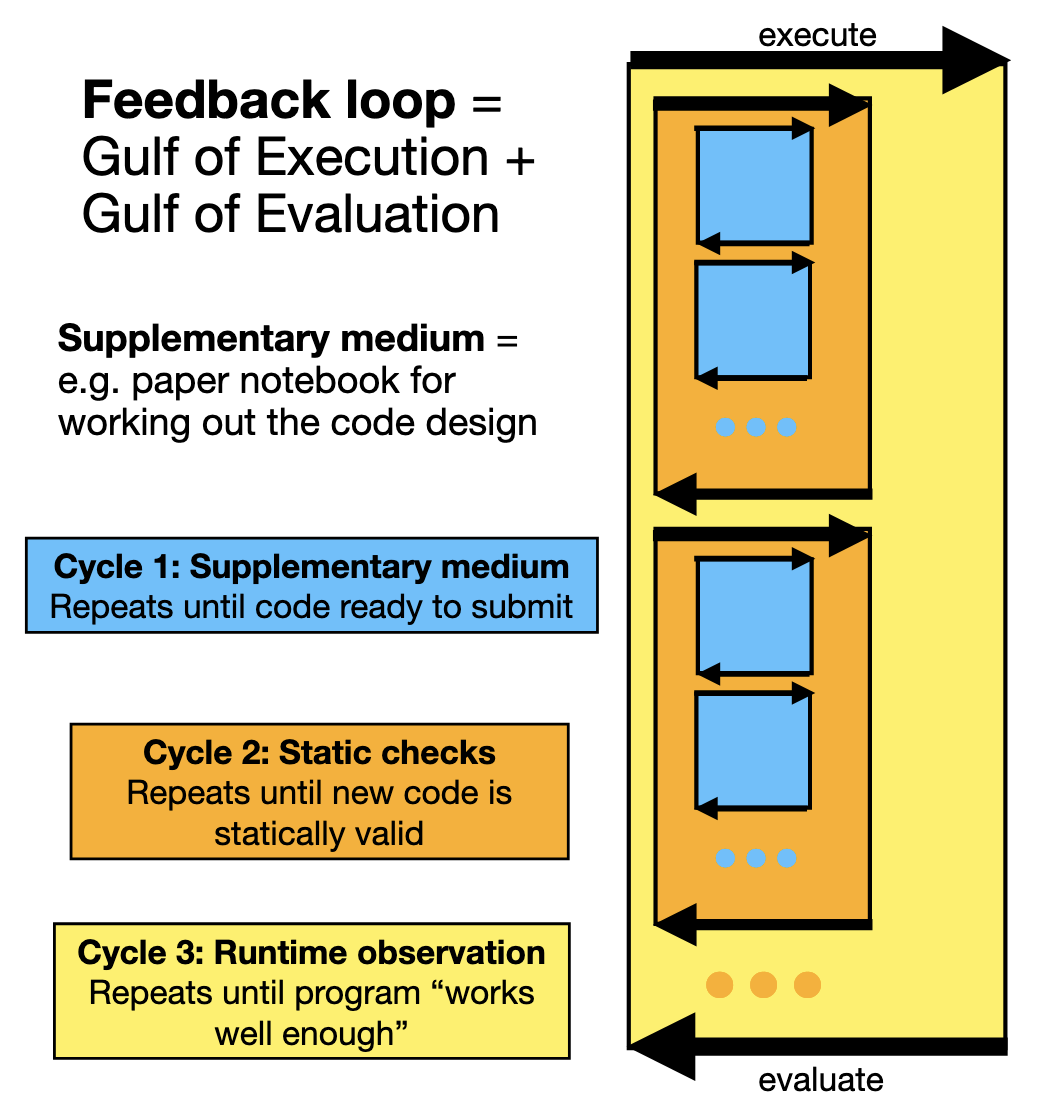
\includegraphics[width=0.5\linewidth]{feedback-loops.png}
  \caption{The nested feedback loops of a statically-checked programming language.\label{fig:feedback-loops}}
\end{figure}

For example, we can analyze statically checked \emph{programming
languages} (e.g.~Java, Haskell) into several feedback loops (Figure
\ref{fig:feedback-loops}):

\begin{enumerate}
\def\labelenumi{\arabic{enumi}.}
\item
  Programmers often think about design details and calculations on a
  whiteboard or notebook, even before writing code. This
  \emph{supplementary medium} has its own feedback loop, even though
  this is often not automatic.
\item
  The code is written and is then put through the static checker. An
  error sends the user back to writing code. In the case of success,
  they are ``allowed'' to run the program, leading into cycle 3.

  \begin{itemize}
  \tightlist
  \item
    The execution gulf comprises multiple cycles of the supplementary
    medium, plus whatever overhead is needed to invoke the compiler
    (such as build systems).
  \item
    The evaluation gulf is essentially the waiting period before static
    errors or a successful termination are observed. Hence this is
    bounded by some function of the length of the code (the same cannot
    be said for the following cycle 3.)
  \end{itemize}
\item
  With a runnable program, the user now evaluates the \emph{runtime}
  behavior. Runtime errors can send the user back to writing code to be
  checked, or to tweak dynamically loaded data files in a similar cycle.

  \begin{itemize}
  \tightlist
  \item
    The execution gulf here may include multiple iterations of cycle 2,
    each with its own nested cycle 1.
  \item
    The \emph{evaluation} gulf here is theoretically unbounded; one may
    have to wait a very long time, or create very specific conditions,
    to rule out certain bugs (like race conditions) or simply to
    consider the program as fit for purpose.
  \item
    By imposing \emph{static checks}, some bugs can be pushed earlier to
    the evaluation stage of cycle 2, reducing the likely size of the
    cycle 3 \emph{evaluation} gulf.
  \item
    On the other hand, this can make it harder to write statically valid
    code, which may increase the number of level-2 cycles, thus
    increasing the total \emph{execution} gulf at level 3.
  \item
    Depending on how these balance out, the total top-level feedback
    loop may grow longer or shorter.
  \end{itemize}
\end{enumerate}

\hypertarget{example-immediate-feedback}{%
\subsubsection{Example: immediate
feedback}\label{example-immediate-feedback}}

The specific case where the \emph{evaluation} gulf is minimized to be
imperceptible is known as \emph{immediate feedback}. Once the user has
caused some change to the system, its effects (including errors) are
immediately visible. This is a key ingredient of \emph{liveness}, though
it is not sufficient on its own. (See \emph{Relations})

The ease of achieving immediate feedback is obviously constrained by the
computational load of the user's effects on the system, and the system's
performance on such tasks. However, such ``loading time'' is not the
only way feedback can be delayed: a common situation is where the user
has to manually ask for (or ``poll'') the relevant state of the system
after their actions, even if the system finished the task quickly. Here,
the feedback could be described as \emph{immediate upon demand} yet not
\emph{automatically demanded}. For convenience, we choose to include the
latter criterion---automatic demand of result---in our definition of
immediate feedback.

In a \emph{REPL} or \emph{shell}, there is a \emph{main} cycle of typing
commands and seeing their output, and a \emph{secondary} cycle of typing
and checking the command line itself. The output of commands can be
immediate, but usually reflects only part of the total effects or even
none at all. The user must manually issue further commands afterwards,
to check the relevant state bit by bit. The secondary cycle, like all
typing, provides immediate feedback in the form of character ``echo'',
but things like syntax errors generally only get reported \emph{after}
the entire line is submitted. This evaluation gulf has been reduced in
the JavaScript console of web browsers, where the line is ``run'' in a
limited manner on every keystroke. Simple commands without
side-effects,\footnote{Of course, these are detected via some
  conservative over-approximation which excludes expressions that
  \emph{might} side-effect.} such as calls to pure functions, can give
instantly previewed results---though partially typed expressions and
syntax errors will not trigger previews.

\hypertarget{example-direct-manipulation}{%
\subsubsection{Example: direct
manipulation}\label{example-direct-manipulation}}

Direct manipulation \cite{DirectManip} is a special case of an immediate
feedback loop. The user sees and interacts with an artefact in a way
that is as similar as possible to real life; this typically includes
dragging with a cursor or finger in order to physically move a visual
item, and is limited by the particular haptic technology in use.

Naturally, because moving real things with one's hands does not involve
any waiting for the object to ``catch up'',\footnote{In some situations,
  such as steering a boat with a rudder, there is a delay between input
  and effect. But on closer inspection, this delay is between the rudder
  and the boat; we do not see the hand pass through the wheel like a
  hologram, followed by the wheel turning a second later. In real life,
  objects touched directly give immediate feedback; objects controlled
  further down the line might not!} direct manipulation is necessarily
an immediate-feedback cycle. If, on the other hand, one were to move a
figure on screen by typing new co-ordinates in a text box, then this
could still give \emph{immediate feedback} (if the update appears
instant and automatic) but would \emph{not} be an example of direct
manipulation.

\emph{Spreadsheets} contain a feedback loop for direct manipulation of
values and formatting, as in any other WYSIWYG application. Here, there
is feedback for every character typed and every change of style. This is
not the case in the other loop for formula editing and formula
invocation. There, we see a larger execution gulf for designing and
typing formulas, where feedback is only given upon committing the
formula by pressing enter. This makes it an ``immediate feedback'' loop
only \emph{on-demand}, as defined above.

\hypertarget{dimension-modes-of-interaction}{%
\subsubsection{Dimension: modes of
interaction}\label{dimension-modes-of-interaction}}

The possible interactions in a programming system are typically
structured so that interactions, and the associated feedback loops, are
only available in certain \emph{modes}. For example, when creating a new
project, the user may be able to configure the project through a
conversational interface like \texttt{npm\ init} in modern JavaScript.
Such interactions are no longer available once the project is created.
This idea of interaction modes goes beyond just programming systems,
appearing in software engineering methodologies. In particular, having a
separate \emph{implementation} and \emph{maintenance} phase would be an
example of two modes.

\emph{Editing vs debugging.} A good example is the distinction between
\emph{editing} and \emph{debugging} mode. When debugging a program, the
user can modify the program state and get (more) immediate feedback on
what individual operations do. In some systems, one can even modify the
program itself during debugging. Such feedback loops are not available
outside of debugging mode.

\emph{Lisp systems} sometimes distinguish between \emph{interpreted} and
\emph{compiled} mode. The two modes do not differ just in the efficiency
of code execution, but also in the interactions they enable. In the
interpreted mode, code can be tested interactively and errors may be
corrected during the code execution (see \emph{Error response}). In the
compiled mode, the program can only be tested as a whole. The same two
modes also exist, for example, in some Haskell systems where the REPL
uses an interpreter (GHCi) distinct from the compiler (GHC).

\emph{Jupyter notebooks.} A programming system may also unify modes that
are typically distinct. The Jupyter notebook environment does not have a
distinct debugging mode; the user runs blocks of code and receives the
result. The single mode can be used to quickly try things out, and to
generate the final result, partly playing the role of both debugging and
editing modes. However, even Jupyter notebooks distinguish between
editing a document and running code.

\hypertarget{dimension-abstraction-construction}{%
\subsubsection{Dimension: abstraction
construction}\label{dimension-abstraction-construction}}

A necessary activity in programming is going between abstract schemas
and concrete instances. Abstractions can be constructed from concrete
examples, first principles or through other methods. A part of the
process may happen in the programmer's mind: they think of concrete
cases and come up with an abstract concept, which they then directly
encode in the system. Alternatively, a system can support these
different methods directly.

One option is to construct abstractions \emph{from first principles}.
Here, the programmer starts by defining an abstract entity such as an
interface in object-oriented programming languages. To do this, they
have to think what the required abstraction will be (in the mind) and
then encode it (in the system).

Another option is to construct abstractions \emph{from concrete cases}.
Here, the programmer uses the system to solve one or more concrete
problems and, when they are satisfied, the system guides them in
creating an abstraction based on their concrete case(s). In a
programming language IDE this manifests as the ``extract function''
refactor, whereas in other systems we see approaches like macro
recording.

\emph{Pygmalion.} In Pygmalion \cite{Pygmalion}, all programming is done
by manipulating concrete icons that represent concrete things. To create
an abstraction, you can use ``Remember mode'', which records the
operations done on icons and makes it possible to bind this recording to
a new icon.

\emph{Jupyter notebook.} In Jupyter notebooks, you are inclined to work
with concrete things, because you see previews after individual cells.
This discourages creating abstractions, because then you would not be
able to look inside at such a fine grained level.

\emph{Spreadsheets.} Up until the recent introduction of lambda
expressions into Excel, spreadsheets have been relentlessly concrete,
without any way to abstract and reuse patterns of computation other than
copy-and-paste.

\hypertarget{relations}{%
\subsubsection{Relations}\label{relations}}

\begin{itemize}
\tightlist
\item
  \emph{Errors} (Section \ref{errors}) A longer evaluation gulf delays
  the detection of errors. A longer execution gulf can increase the
  \emph{likelihood} of errors (e.g.~writing a lot of code or taking a
  long time to write it). By turning runtime bugs into statically
  detected bugs, the combined evaluation gulfs can be reduced.
\item
  \emph{Adoptability} (Section \ref{adoptability}): The \emph{execution}
  gulf is concerned with software using and programming in general. The
  time taken to realize an idea in software is affected by the user's
  familiarity and the system's \emph{learnability}.
\item
  \emph{Notation} (Section \ref{notation}): Feedback loops are related
  to \emph{notational structures}. In a system with multiple notations,
  each notation may have different associated feedback loops. The motto
  ``The thing on the screen is supposed to be the actual thing''
  \cite{NakedObjects}, adopted in the context of live programming,
  relates \emph{liveness} to a direct connection between surface and
  internal notations. The idea is that interactable objects should be
  equipped with faithful behavior, instead of being intangible shadows
  cast by the hidden \emph{real} object.
\end{itemize}

\hypertarget{notation}{%
\subsection{Notation}\label{notation}}

\mybox{How are the different textual / visual programming notations related?}

Programming is always done through some form of notation. We consider
notations in the most general sense and include any structured gesture
using textual or visual notation. Textual notations primarily include
programming languages, but also things like configuration files. Visual
notations include graphical programming languages. Other kinds of
structured gestures include user interfaces for constructing visual
elements used in the system.

\hypertarget{dimension-notational-structure}{%
\subsubsection{Dimension: notational
structure}\label{dimension-notational-structure}}

In practice, most programming systems use multiple notations. Different
notations can play different roles in the system. On the one hand,
multiple \emph{overlapping notations} can be provided as different ways
of programming the same aspects of the system. In this case, each
notation may be more suitable to different kinds of users, but may have
certain limitations (for example, a visual notation may have a limited
expressive power). On the other hand, multiple \emph{complementing
notations} may be used as the means for programming different aspects of
the system. In this case, programming the system requires using multiple
notations, but each notation may be more suitable for the task at hand;
think of how HTML describes document structure while JavaScript
specifies its behavior.

\hypertarget{example-overlapping-notations}{%
\subsubsection{Example: overlapping
notations}\label{example-overlapping-notations}}

A programming system may provide multiple notations for programming the
same aspect of the system. This is typically motivated by an attempt to
offer easy ways of completing different tasks: say, a textual notation
for defining abstractions and a visual notation for specifying concrete
structures. The crucial issue in this kind of arrangement is
\emph{synchronizing} the different notations; if they have different
characteristics, this may not be a straightforward mapping. For example,
source code may allow more elaborate abstraction mechanisms like loops,
which will appear as visible repetition in the visual notation. What
should such a system do when the user edits a single object that
resulted from such repetition? Similarly, textual notation may allow
incomplete expressions that do not have an equivalent in the visual
notation. For programming systems that use \emph{overlapping notations},
we need to describe how the notations are synchronized.

\emph{Sketch-n-Sketch} \cite{SnS} employs overlapping notations for
creating and editing SVG and HTML documents. The user edits documents in
an interface with a split-screen structure that shows source code on the
left and displayed visual output on the right. They can edit both of
these and changes are propagated to the other view. The code can use
abstraction mechanisms (such as functions) which are not completely
visible in the visual editor (an issue we return to in \emph{expression
geography} below). Sketch-n-Sketch can be seen as an example of a
\emph{projectional editor}.\footnote{Technically, traditional
  projectional editors usually work more directly with the abstract
  syntax tree of a programming
  language.\note{TODO: Insert some more references to research on "projectional editors"}}

\emph{UML Round-tripping.} Another example of a programming system that
utilizes the \emph{overlapping notations} structure are UML design tools
that display the program both as source code and as a UML diagram. Edits
in one result in automatic update of the other. An example is the
Together/J\footnote{https://www.mindprod.com/jgloss/togetherj.html}
system. To solve the issue of notation synchronization, such systems
often need to store additional information in the textual notation,
typically using a special kind of code comment. In this example, after
the user re-arranges classes in UML diagrams, the new locations need to
be updated in the code.

\hypertarget{example-complementing-notations}{%
\subsubsection{Example: complementing
notations}\label{example-complementing-notations}}

A programming system may also provide multiple complementing notations
for programming different aspects of its world. Again, this is typically
motivated by the aim to make specifying certain aspects of programming
easier, but it is more suitable when the different aspects can be more
clearly separated. The key issue for systems with complementing
notations is how the different notations are connected. The user may
need to use both notations at the same time, or they may need to
progress from one to the next level when solving increasingly complex
problems. In the latter case, the learnability of progressing from one
level to the next is a major concern.

\emph{Spreadsheets and HyperCard.} In Excel, there are three different
complementing notations that allow users to specify aspects of
increasing complexity: (i) the visual grid, (ii) formula language and
(iii) a macro language such as Visual Basic for Applications. The
notations are largely independent and have different degrees of
expressive power. Entering values in a grid cannot be used for
specifying new computations, but it can be used to adapt or run a
computation, for example when entering different alternatives in What-If
Scenario Analysis. More complex tasks can be achieved using formulas and
macros. A user gradually learns more advanced notations, but experience
with a previous notation does not help with mastering the next one. The
approach optimizes for easy learnability at one level, but introduces a
hurdle for users to surmount in order to get to the second level. The
notational structure of \emph{HyperCard} is similar and consists of (i)
visual design of cards, (ii) visual programming (via the GUI) with a
limited number of operations and (iii) HyperTalk for arbitrary
scripting.

\emph{Boxer and Jupyter.} Boxer \cite{Boxer} uses \emph{complementing
notations} in that it combines a visual notation (the layout of the
document and the boxes of which it consists) with textual notation (the
code in the boxes). Here, the textual notation is always nested within
the visual. The case of Jupyter notebooks is similar. The document
structure is graphical; code and visual outputs are nested as editable
cells in the document. This arrangement is common in many other systems
such as Flash or Visual Basic, which both combine visual notation with
textual code, although one is not nested in the other.

\hypertarget{dimensions-surface-notation-and-internal-notation}{%
\subsubsection{Dimensions: surface notation and internal
notation}\label{dimensions-surface-notation-and-internal-notation}}

All programming systems build up structures in memory, which we can
consider as an \emph{internal notation} not usually visible to the user.
Even though such structures might be revealed in a debugger, they are
hidden during normal operation. What the user interacts with instead is
the \emph{surface notation}, typically one of text or shapes on a
screen. Every interaction with the surface notation alters the internal
notation in some way, and the nature of this connection is worth
examining in more detail. To do this, we illustrate with a simplified
binary choice for the form of these notations.

\hypertarget{examples-implicit-vs.-explicit-structure}{%
\subsubsection{Examples: implicit vs.~explicit
structure}\label{examples-implicit-vs.-explicit-structure}}

Let us partition notations into two families. Notations with
\emph{implicit structure} present as a sequence of items, such as
textual characters or audio signal amplitudes. Those with \emph{explicit
structure} present as a tree or graph without an obvious order, such as
shapes in a vector graphics editor. These two types of notations can be
transformed into each other: the implicit structure contained in a
string can be \emph{parsed} into an explicit syntax tree, and an
explicit document structure might be \emph{rendered} into a sequence of
characters with the same implicit structure.

Now consider an interface to enter a personal name made up of a forename
and a surname. For the surface notation, there could be a single text
field to hold the names separated with a space; here, the sub-structure
is implicit in the string. Alternatively, there could be two fields
where the names are entered separately, and their separation is
explicit. A similar choice exists for the internal notation built up in
memory: is it a single string, or two separate strings?

We can see that these choices give four combinations. More
interestingly, they exhibit unique characters owing to two key
asymmetries. Firstly, surface notation is mostly used by humans, while
the internal notation is mostly used by the computer. Secondly, and most
significantly, computer programs can only work with explicit structure,
while humans can understand both explicit and implicit structure.
\joel{informal vs formal structure?} Because of the practical
consequences of this asymmetry, we will examine the combinations with
emphasis on the \emph{internal} notation first.

\hypertarget{examples-one-string-in-memory-implicitly-structured-internal-notation}{%
\subsubsection{Examples: one string in memory (implicitly structured
internal
notation)}\label{examples-one-string-in-memory-implicitly-structured-internal-notation}}

The simplest case here would be with implicit structure in the surface
notation, i.e.~a single text box for the full name. Edits to the surface
are straightforwardly mirrored interally and persisted to disk. This
corresponds to \emph{text editing}. We can generalize this to an idea of
\emph{sequence editing} if we view the fundamental act as
\emph{recording} events to a list over time. For text, these are key
presses; for an audio editing interface they would be samples of sound
amplitude.

In the other case, with two text boxes, we have \emph{sequence
rendering}. The information about the separation of the two strings,
present in the interface, is not quite ``thrown away'' but is made
\emph{implicit} as a space character in the string. This combination
corresponds to Visual Basic generating code from GUI forms, video
editors combining multiple clips and effects into a single stream, and
3D renderers turning scene graphs into pixels. Another example is
line-based diff tools, which provide side-by-side views and related
interfaces, yet must ultimately forward the user's changes to the
underlying text file.

Critically, in both of these cases, a computer program can only
manipulate the stored sequences \emph{as} sequences; that is, by
inserting, removing, or serially reading. The appealing feature here is
that these operations are simple to implement and may be re-usable
across many types of sequences. However, any further structure is
implicit and, to work with it programmatically, a user must write a
program to \emph{parse} it into something explicit. Furthermore, errors
introduced at this stage may simply be \emph{recorded} into the
sequence, only to be discovered much later in an attempt to use the
data.

\hypertarget{examples-two-strings-in-memory-explicitly-structured-internal-notation}{%
\subsubsection{Examples: two strings in memory (explicitly structured
internal
notation)}\label{examples-two-strings-in-memory-explicitly-structured-internal-notation}}

\joel{TODO: cite The Many Forms of a Single Fact}

With two text boxes, both notations match, so there is not much work to
do. As with sequence editing, edits on the surface can be mirrored to
the internal notation. This corresponds to vector graphics editors and
3D modelling tools, as well as \emph{structure editors} for programming
languages. For this reason we call this combination \emph{structure
editing}.

With a single text field, we have \emph{structure recovery.} Parsing
needs to happen each time the input changes. This style is found in the
DOM inspector in browser developer tools, where HTML can be edited as
text to make changes to the document tree structure. More generally,
this is the mode found in compilers and interpreters which accept
program source text yet internally work on tree and graph structures. It
is also possible to do a sort of structure editing this way, where the
experience is made to resemble text editing but the output is explicitly
structured.

In both of these cases, in order to write programs to transform,
analyze, or otherwise work with the digital artefact the user has
created, one can trivially navigate the stored structure instead of
parsing it for every use. Parsing is either done away with altogether or
is reduced to a transient process that happens during editing; this
means errors can be caught at the moment they are introduced instead of
remaining latent.

\hypertarget{dimension-primary-and-secondary-notations}{%
\subsubsection{Dimension: primary and secondary
notations}\label{dimension-primary-and-secondary-notations}}

In practice, most programming systems use multiple notations. Even in
systems based on traditional programming languages, the \emph{primary
notation} of the language is often supported by \emph{secondary
notations} such as annotations encoded in comments and build tool
configuration files. However, it is possible for multiple notations to
be primary, especially if they are \emph{overlapping} as defined
earlier.

\emph{Programming languages.} Programming systems built around
traditional programming languages typically have further notations or
structured gestures associated with them. The primary notation in UNIX
is the C programming language. Yet this is enclosed in a programming
\emph{system} providing a multi-step mechanism for running C code via
the terminal, assisted by secondary notations such as shell scripts.
Some programming systems attempt to integrate tools that normally rely
on secondary notations into the system itself, reducing the number of
secondary notations that the programmer needs to master. For example, in
the Smalltalk descendant Pharo, versioning and package management is
done from within Pharo, removing the need for secondary notation such as
\texttt{git} commands and dependency configuration files.\footnote{The
  tool for versioning and package management in Pharo can still be seen
  as an \emph{internal} domain-specific language and thus as a secondary
  notation, but its basic structure is \emph{shared} with other
  notations in the Pharo system.}

\emph{Haskell.} In Haskell, the primary notation is the programming
language, but there are also a number of secondary notations. Those
include package managers (e.g.~the \texttt{cabal.project} file) or
configuration files for Haskell build tools. More interestingly, there
is also an informal mathematical notation associated with Haskell that
is used when programmers discuss programs on a whiteboard or in academic
publications. The idea of having such a mathematical notation dates back
to the \emph{Report on Algol 58} \cite{Alg58}, which explicitly defined
a ``publication language'' for ``stating and communicating problems''
using Greek letters and subscripts.

\hypertarget{dimension-expression-geography}{%
\subsubsection{Dimension: expression
geography}\label{dimension-expression-geography}}

A crucial feature of a notation is the relationship between the
structure of the notation and the structure of the behavior it encodes.
Most importantly, do \emph{similar expressions} in a particular notation
represent \emph{similar behavior}?\footnote{See Basman's
  \cite{NotYetCraft} similar discussion of ``density''.} Visual
notations may provide a more or less direct mapping. On the one hand,
similar-looking code in a block language may mean very different things.
On the other hand, similar looking design of two HyperCard cards will
result in similar looking cards---the mapping between the notation and
the logic is much more direct.

\emph{C/C++ expression language.} In textual notations, this may easily
not be the case. Consider the two C conditionals:

\begin{itemize}
\tightlist
\item
  \texttt{if\ (x==1)\ \{\ ...\ \}} evaluates the Boolean expression
  \texttt{x==1} to determine whether \texttt{x} equals \texttt{1},
  running the code block if the condition holds.
\item
  \texttt{if\ (x=1)\ \{\ ...\ \}} \emph{assigns} \texttt{1} to the
  variable \texttt{x}. In C, assignment is an expression
  \emph{returning} the assigned value, so the result \texttt{1} is
  interpreted as \texttt{true} and the block of code is \emph{always}
  executed.
\end{itemize}

A notation can be designed to map better to the logic behind it, for
example, by requiring the user to write \texttt{1==x}. This solves the
above problem as \texttt{1} is a literal rather than a variable, so it
cannot be assigned to (\texttt{1=x} is a compile error).

\hypertarget{dimension-uniformity-of-notations}{%
\subsubsection{Dimension: uniformity of
notations}\label{dimension-uniformity-of-notations}}

One common concern with notations is the extent to which they are
uniform. A uniform notation can express a wide range of things using
just a small number of concepts. The primary example here is
S-expressions from Lisp. An S-expression is either an atom or a pair of
S-expressions written \texttt{(s1\ .\ s2)}. By convention, an
S-expression \texttt{(s1\ .\ (s2\ .\ (s3\ .\ nil)))} represents a list,
written as \texttt{(s1\ s2\ s3)}. In Lisp, uniformity of notations is
closely linked to uniformity of representation.\footnote{Notations
  generally are closely linked to representation in that the notation
  may mirror the structures used for program representation. Basman et
  al.~\cite{Externalize} refer to this as a distinction between ``dead''
  notation and ``live'' representation forms).} In the idealized model
of LISP 1.5, the data structures represented by an S-expression are what
exists in memory. In real-world Lisp systems, the representation in
memory is more complex. A programming system can also take a very
different approach and fully separate the notation from the in-memory
representation.

\emph{Lisp systems.} In Lisp, source code is represented in memory as
S-expressions, which can be manipulated by Lisp primitives. In addition,
Lisp systems have robust macro processing as part of their semantics:
expanding a macro revises the list structure of the code that uses the
macro. Combining these makes it possible to define extensions to the
system in Lisp, with syntax indistinguishable from Lisp. Moreover, it is
possible to write a program that constructs another Lisp program and not
only run it interpretively (using the \texttt{eval} function) but
compile it at runtime (using the \texttt{compile} function) and execute
it. Many domain-specific languages, as well as prototypes of new
programming languages (such as Scheme), were implemented this way. Lisp
the language is, in this sense, a ``programmable programming language''.
\cite{LispIntro,ProgProgLang}

\hypertarget{references}{%
\subsubsection{References}\label{references}}

\emph{Cognitive Dimensions of Notation} \cite{CogDims} provide a
comprehensive framework for analysing individual notations, while our
focus here is on how multiple notations are related and how they are
structured. It is worth noting that the Cognitive Dimensions also define
\emph{secondary notation}, but in a different sense to ours. For them,
secondary notation refers to whether a notation allows including
redundant information such as color or comments for readability
purposes.

The importance of notations in the practice of science, more generally,
has been studied by \cite{PaperTools} as ``paper tools''. These are
formula-like entities which can be manipulated by humans in lieu of
experimentation, such as the aforementioned mathematical notation in
Haskell: a ``paper tool'' for experimentation on a whiteboard.
Programming notations are similar, but they are a way of communicating
with a machine; the experimentation does not happen on paper alone.

\hypertarget{relations-1}{%
\subsubsection{Relations}\label{relations-1}}

\begin{itemize}
\tightlist
\item
  \emph{Interaction} (Section \ref{interaction}): The feedback loops
  that exist in a programming system are typically associated with
  individual notations. Different notations may also have different
  feedback loops.
\item
  \emph{Adoptability} (Section \ref{adoptability}): Notational structure
  can affect learnability. In particular, complementing notations may
  require (possibly different) users to master multiple notations.
  Overlapping notations may improve learnability by allowing the user to
  edit the program in one way (perhaps visually) and see the effect in
  the other notation (such as code.)
\item
  \emph{Errors} (Section \ref{errors}). A process that merely records
  user actions in a sequence (such as text editing) will, in particular,
  record any \emph{errors} the user makes and defer their handling to
  later use of the data, keeping the errors \emph{latent}. A process
  which instead treats user actions as edits to a structure, with
  constraints and correctness rules, will be able to catch errors at the
  moment they are introduced and ensure the data coming out is
  error-free.
\end{itemize}

\hypertarget{conceptual-structure}{%
\subsection{Conceptual Structure}\label{conceptual-structure}}

\mybox{How is meaning constructed? How are internal and external incentives balanced?}

\hypertarget{dimension-conceptual-integrity-vs.-openness}{%
\subsubsection{Dimension: conceptual integrity
vs.~openness}\label{dimension-conceptual-integrity-vs.-openness}}

The evolution of programming systems has led away from \emph{conceptual
integrity} towards an intricate ecosystem of specialized technologies
and industry standards. Any attempt to unify parts of this ecosystem
into a coherent whole will create \emph{incompatibility} with the
remaining parts, which becomes a major barrier to adoption. Designers
seeking adoption are pushed to focus on localized incremental
improvements that stay within the boundaries established by existing
practice. This creates a tension between how highly they can afford to
value conceptual elegance, and how open they are to the pressures
imposed by society. We will turn to both of these opposite
ends---\emph{integrity} and \emph{openness}---in more detail.

\hypertarget{example-conceptual-integrity}{%
\subsubsection{Example: conceptual
integrity}\label{example-conceptual-integrity}}

\begin{quote}
I will contend that Conceptual Integrity is the most important
consideration in system design. It is better to have a system omit
certain anomalous features and improvements, but to reflect one set of
design ideas, than to have one that contains many good but independent
and uncoordinated ideas. (Fred~Brooks, \emph{Aristocracy, Democracy and
System Design} \cite{brooks95aristo})
\end{quote}

\note{The essence of this style can be captured by the phrase “the right thing”. To such a designer it is important to get all of the following characteristics right: Simplicity … Correctness … Consistency … Completeness --- Richard Gabriel}

\begin{quote}
Conceptual integrity arises not (simply) from one mind or from a small
number of agreeing resonant minds, but from sometimes hidden co-authors
and the thing designed itself. (Richard ~Gabriel, \emph{Designed As
Designer} \cite{DesignedAsDesigner})
\end{quote}

Conceptual integrity strives to reduce complexity at the source; it
employs \emph{unified concepts} that may \emph{compose orthogonally} to
generate diversity. Perhaps the apotheosis of this approach can be found
in early Smalltalk and Lisp machines, which were complete programming
systems built around a single language. They incorporated capabilities
commonly provided \emph{outside} the programming language by operating
systems and databases. Everything was done in one language, and so
everything was represented with the datatypes of that language. Likewise
the libraries and idioms of the language were applicable in all
contexts. Having a \emph{lingua franca} avoided much of the friction and
impedance mismatches inherent to multi-language systems. A similar drive
exists in the Python programming language, which follows the principle
that ``There should be one---and preferably only one---obvious way to do
it'' in order to promote community consensus on a single coherent style.

In addition to Smalltalk and Lisp, many programming languages focus on
one kind of data structure \cite{MemMod}:

\begin{itemize}
\tightlist
\item
  In COBOL, data consists of nested records as in a business form.
\item
  In Fortran, data consists of parallel arrays.
\item
  In SQL, data is a set of relations with key constraints.
\item
  In scripting languages like Python, Ruby, and Lua, much data takes the
  form of string-indexed hash tables.
\end{itemize}

Finally, many languages are \emph{imperative}, staying close to the
hardware model of addressable memory, lightly abstracted into primitive
values and references into mutable arrays and structures. On the other
hand, \emph{functional} languages hide references and treat everything
as immutable structured values. This conceptual simplification benefits
certain kinds of programming, but can be counterproductive when an
imperative approach is more natural, such as in external input/output.

\hypertarget{example-conceptual-openness}{%
\subsubsection{Example: conceptual
openness}\label{example-conceptual-openness}}

\emph{Perl, contra Python}. In contrast to Python's outlook, Perl
proclaims ``There is more than one way to do it'' and considers itself
``the first postmodern programming language'' \cite{Perl}. ``Perl
doesn't have any agenda at all, other than to be maximally useful to the
maximal number of people. To be the duct tape of the Internet, and of
everything else.'' The Perl way is to accept the status quo of evolved
chaos and build upon it using duct tape and ingenuity. Taken to the
extreme, a programming system becomes no longer a \emph{system},
properly speaking, but rather a \emph{toolkit for improvising}
assemblages of \emph{found} software. Perl can be seen as championing
the values of \emph{pluralism}, \emph{compatibility}, or
\emph{conceptual openness} over conceptual integrity. This philosophy
has been called \emph{Postmodern Programming} \cite{PoMoProNotes}.

\emph{C++, contra Smalltalk}. Another case is that of C++, which added
to C the Object-Oriented concepts developed by Smalltalk while remaining
100\% compatible with C, down to the level of ABI and performance. This
strategy was enormously successful for adoption, but came with the
tradeoff of enormous complexity compared to languages designed from
scratch for OO, like Smalltalk, Ruby, and Java.

\emph{Worse, contra Better}. Richard Gabriel first described this
dilemma in his influential 1991 essay \emph{Worse is Better} \cite{WIB}
analyzing the defeat of Lisp by UNIX and C. Because UNIX and C were so
easy to port to new hardware, they were ``the ultimate computer
viruses'' despite providing only ``about 50\%--80\% of what you want
from an operating system and programming language''. Their conceptual
openness meant that they adapted easily to the evolving conditions of
the external world. The tradeoff was decreased conceptual integrity,
such as the undefined behaviours of C, the junkyard of working
directories, and the proliferation of special purpose programming
languages to provide a complete development environment.

\tp{Smalltalk objects are "all levels of granularity"; UNIX files are large-scale; Haskell data structures small-scale; very big virtual machines; there is also the web / distributed file system?}

\emph{UNIX and Files}. Many programming languages and systems impose
structure at a ``fine granularity'': that of individual variables and
other data and code structures. Conversely, systems like UNIX and the
Web impose fewer restrictions on how programmers represent things. UNIX
insists only on a basic infrastructure of ``large objects''
\cite{KellOS}, delegating all fine-grained structure to client programs.
This scores many points for conceptual openness. \emph{Files} provide a
universal API for reading and writing byte streams, a low-level
construct containing so many degrees of freedom that it can support a
wide variety of formats and ecosystems. \emph{Processes} similarly
provide a thin abstraction over machine-level memory and processors.

Concepual integrity is necessarily sacrificed for such openness; while
``everything is a file'' gestures at integrity, in the vein of
Smalltalk's ``everything is an object'', exceptions proliferate.
Directories are special kinds of files with special operations, hardware
device files require special \texttt{ioctl} operations, and many
commands expect files containing newline separators. Additionally,
because client programs must supply their \emph{own} structure for
fine-grained data and code, they are given little in the way of mutual
compatibility. As a result, they tend to evolve into competing silos of
duplicated infrastructure \cite{KellOS,Mythical}.

\emph{The Web}. Web HTTP endpoints, meanwhile, have proven to be an even
more adaptable and viral abstraction than UNIX files. They operate at a
similar level of abstraction as files, but support richer content and
encompass internet-wide interactions between autonomous systems. In a
sense, HTTP GET and PUT have become the ``subroutine calls'' of an
internet-scale programming system. Perhaps the most salient thing about
the Web is that its usefulness came as such a surprise to everyone
involved in designing or competing with it. It is likely that, by
staying close to the existing practice of transferring files, the Web
gained a competitive edge over more ambitious and less familiar
hypertext projects like Xanadu \cite{TedNelson}.

The choice between compatibility and integrity correlates with the
personality traits of \emph{pragmatism} and \emph{idealism}. It is
pragmatic to accept the status quo of technology and make the best of
it. Conversely, idealists are willing to fight convention and risk
rejection in order to attain higher goals. We can wonder which came
first: the design decision or the personality trait? Do Lisp and Haskell
teach people to think more abstractly and coherently, or do they filter
for those with a pre-existing condition? Likewise, perhaps introverted
developers prefer the cloisters of Smalltalk or Lisp to the adventurous
``Wild West'' of the Web.

\hypertarget{dimension-composability}{%
\subsubsection{Dimension: composability}\label{dimension-composability}}

In short, \emph{you can get anywhere by putting together a number of
smaller steps.} There exist building blocks which span a range of useful
combinations.
\note{JE. LEGOs might be a more friendly example than Linear Algebra.
Such a property can be analogized to *linear independence* in mathematical vector spaces: a number of primitives (basis vectors) whose possible combinations span a meaningful space.}
Composability is, in a sense, key to the notion of ``programmability''
and every programmable system will have some level of composability
(e.g.~in the scripting language.)

\emph{UNIX} shell commands are a standard example of composability. The
base set of primitive commands can be augmented by programming command
executables in other languages. Given some primitives, one can ``pipe''
one's output to another's input (\texttt{\textbar{}}), sequence
(\texttt{;} or \texttt{\&\&}), select via conditions, and repeat with
loop constructs, enabling full imperative programming. Furthermore,
command compositions can be packaged into a named ``script'' which
follows the same interface as primitive commands, and named subprograms
within a script can also be defined.

In \emph{HyperCard}, the \emph{Authoring Environment} is
\emph{non}-composable for programming buttons: there is simply a set of
predefined behaviors to choose from. Full scriptability is available
only in the \emph{Programming Environment}.

The \emph{Haskell type system}, as well as that of other functional
programming languages, exhibits high composability. New types can be
defined in terms of existing ones in several ways. These include
records, discriminated unions, function types and recursive constructs
(e.g.~to define a \texttt{List} as either a \texttt{Nil} or a
combination of element plus other list.) The C programming language also
has some means of composing types that are analogous in some ways, such
as structs, unions, enums and indeed even function pointers. For every
type, there is also a corresponding ``pointer'' type. It lacks, however,
the recursive constructs permitted in Haskell types.

\note{*Web* Mashups in Web 2.0? Yahoo Pipes?}

\hypertarget{dimension-convenience}{%
\subsubsection{Dimension: convenience}\label{dimension-convenience}}

In short, \emph{you can get to X, Y or Z via one single step.} There are
ready-made solutions to specific problems, not necessarily generalizable
or composable. Convenience often manifests as ``canonical'' solutions
and utilities in the form of an expansive standard library.

Composability without convenience is a set of atoms or gears;
theoretically, anything one wants could be built out of them, but one
must do that work. This situation has been criticized as the \emph{Lisp
Curse} \cite{LispCurse}.

Composability \emph{with} convenience is a set of convenient specific
tools \emph{along with} enough components to construct new ones. The
specific tools themselves could be transparently composed of these
building blocks, but this is not essential. They save users the time and
effort it would take to ``roll their own'' solutions to common tasks.

For example, let us turn to a convenience factor of \emph{UNIX} shell
commands, having already discussed their composability above. Observe
that it would be possible, in principle, to pass all information to a
program via standard input. Yet in actual practice, for convenience,
there is a standard interface of \emph{command-line arguments} instead,
separate from anything the program takes through standard input. Most
programming systems similarly exhibit both composability and
convenience, providing templates, standard libraries, or otherwise
pre-packaged solutions, which can nevertheless be used programmatially
as part of larger operations.

\note{ex: something in the UI world? one click vs. long winded "principled" way of doing the thing? (macros? applescript?)}

\hypertarget{dimension-commonality}{%
\subsubsection{Dimension: commonality}\label{dimension-commonality}}

\note{JE This seems like data modelling issues that happen during application design, not programming system design.}

Humans can see Arrays, Strings, Dicts and Sets all have a ``size'', but
the software needs to be \emph{told} that they are the ``same''.
Commonality like this can be factored out into an explicit structure (a
``Collection'' class), analogous to database \emph{normalization}. This
way, an entity's size can be queried without reference to its particular
details: if \texttt{c} is declared to be a Collection, then one can
straightforwardly access \texttt{c.size}.

Alternatively, it can be left implicit. This is less upfront work, but
permits instances to \emph{diverge}, analogous to \emph{redundancy} in
databases. For example, Arrays and Strings might end up with ``length'',
while Dict and Set call it ``size''. This means that, to query the size
of an entity, it is necessary to perform a case split according to its
concrete type, solely to funnel the diverging paths back to the
commonality they represent:

\begin{verbatim}
if (entity is Array or String)  size := entity.length
else if (entity is Dict or Set) size := entity.size
\end{verbatim}

\joel{Web APIs e.g. onmousedown/onmouseup, imperative onmousemove instead of reified mouse pointer observable (this belongs more in a Factoring of Structure / Complexity dimension...)
   - tbh this is also a "machine legibility" issue; a human can recognise onmousemove and onmousedown as having something in common -- "mouse" -- but the computer just sees two non-equal strings as different as zQx6= and omlette.
   - onmousedown further makes the *mouse* part explicit, but the sub-device -- the button -- is passed as a numerical argument. ...
   - What really annoyed me, and seems most relevant, is that mouse buttons and keyboard keys the same in a very significant way -- they're binary-state buttons -- which means they ought to "implement the same interface", so the system will let me treat them the same insofar as they have commonalities like this. It should be trivial to rebind keyboard keys to the mouse buttons or vice versa, but this "poor factoring" obstructs this.
   - viz. OOP interfaces and abstraction, this factoring is forcing you to rely on irrelevant concrete details of the object. Instead of `if (isMouseButton) listenMouseButton(fn) else if (isKey) listenKey(fn)`, it should just be `listen(fn)`.}

\note{
EXAMPLES: interfaces/base classes; structural vs nominal typing
EXAMPLES: non-programming language world?
HyperCard - had shared backgrounds, which arose from the need of writing the help files.
}

\hypertarget{examples-flattening-and-factoring}{%
\subsubsection{Examples: flattening and
factoring}\label{examples-flattening-and-factoring}}

Data structures usually have several ``moving parts'' that can vary
independently. For example, a simple pair of ``vehicle type'' and
``color'' might have all combinations of (Car, Van, Train) and (Red,
Blue). In this \emph{factored} representation, we can programmatically
change the color directly: \texttt{pair.second\ =\ Red} or
\texttt{vehicle.colour\ =\ Red}.

In some contexts, such as class names, a system might only permit such
multi-dimensional structure as an \emph{exhaustive enumeration}: RedCar,
BlueCar, RedVan, BlueVan, RedTrain, BlueTrain, etc. The system sees a
flat list of atoms, even though a human can see the sub-structure
encoded in the string. In this world, we cannot simply ``change the
color to Red'' programmatically; we would need to case-split as follows:

\begin{verbatim}
if (type is BlueCar) type := RedCar
else if (type is BlueVan) type := RedVan
else if (type is BlueTrain) type := RedTrain
...
\end{verbatim}

The \emph{commonality} between RedCar, RedVan, BlueCar, and so on has
been \emph{flattened}. There is implicit structure here that remains
\emph{un-factored}, similar to how numbers can be expressed as singular
expressions (16) or as factor products (2,2,2,2). \emph{Factoring} this
commonality gives us the original design, where there is a pair of
values from different sets.

In \emph{relational databases}, there is an opposition between
\emph{normalization} and \emph{redundancy}. In order to fit multi-table
data into a \emph{flat} table structure, data needs to be duplicated
into redundant copies. When data is \emph{factored} into small tables as
much as possible, such that there is only one place each piece of data
``lives'', the database is in \emph{normal form} or \emph{normalized}.
Redundancy is useful for read-only processes, because there is no need
to join different tables together based on common keys. Writing,
however, becomes risky; in order to modify one thing, it must be
synchronized to the multiple places it is stored. This makes highly
normalized databases optimized for writes over reads.

\hypertarget{remark-the-end-of-history}{%
\subsubsection{Remark: the end of
history?}\label{remark-the-end-of-history}}

Today we live in a highly developed world of software technology. It is
estimated that 41,000 person years have been invested into Linux. We
describe software development technologies in terms of \emph{stacks} of
specialized tools, each of which might capitalize over 100 person-years
of development. Programming systems have become programming ecosystems:
not designed, but evolved. How can we noticeably improve programming in
the face of the overwhelming edifice of existing technology? There are
strong incentives to focus on localized incremental improvements that
don't cross the established boundaries.

The history of computing is one of cycles of evolution and revolution.
Successive cycles were dominated in turn by mainframes, minicomputers,
workstations, personal computers, and the Web. Each transition built a
whole new technology ecosystem replacing or on top of the previous. The
last revolution, the Web, was 25 years ago, with the result that many
people have never experienced a disruptive platform transition. Has
history stopped, or are we just stuck in a long cycle, with increasingly
pent-up pressures for change? If it is the latter, then incompatible
ideas now spurned may yet flourish.

\hypertarget{references-1}{%
\subsubsection{References}\label{references-1}}

\begin{itemize}
\tightlist
\item
  How to Design a Good API and Why it Matters \cite{APIdesign}
\end{itemize}

\DIFaddbegin \hypertarget{customizability}{%
\subsection{Customizability}\label{customizability}}

\mybox{Once a program exists in the system, how can it be extended and modified?}

\DIFadd{Programming is a gradual process. We start either from nothing, or from
an existing program, and gradually extend and refine it until it serves
a given purpose. Programs created using different programming systems
can be refined to different extents, in different ways, at different
stages of their existence.
}

\DIFadd{Consider three examples. First, a program in a conventional programming
language like Java can be refined only by modifying its source code.
However, you may be able to do so by just adding new code, such as a new
interface implementation. Second, a spreadsheet can be modified at any
time by modifying the formulas or data it contains. There is no separate
programming phase. However, you have to modify the formulas directly in
the cell---there is no way of modifying it by specifying a change in a
way that is external to the cell. Third, a }\emph{\DIFadd{self-sustaining}}
\DIFadd{programming system, such as Smalltalk, does not make an explicit
distinction between ``programming'' and ``using'' phases, and it can be
modified and extended via itself. It gives developers the power to
experiment with the system and, in principle, replace it with a better
system from within.
}

\hypertarget{dimension-staging-of-customization}{%
\subsubsection{Dimension: staging of
customization}\label{dimension-staging-of-customization}}

\DIFadd{For systems that distinguish between different stages, such as writing
source code versus running a program, customization methods may be
different for each stage. In traditional programming languages,
customization is done by modifying or adding source code at the
programming stage, but there is no (automatically provided) way of
customizing the created programs once they are running.
}

\DIFadd{There are a number of interesting questions related to staging of
customization. First, what is the notation used for customization? This
may be the notation in which a program was initially created, but a
system may also use a secondary notation for customization (consider
Emacs using Emacs Lisp). For systems with a stage distinction, an
important question is whether such changes are }\emph{\DIFadd{persistent}}\DIFadd{.
}

\emph{\DIFadd{Smalltalk, Interlisp and similar.}} \DIFadd{In image-based programming
systems, there is generally no strict distinction between stages and so
a program can be customized during execution in the same way as during
development. The program image includes the programming environment.
Users of a program can open this, navigate to a suitable object or a
class (which serve as the }\emph{\DIFadd{addressable extension points}}\DIFadd{) and
modify that. Lisp-based systems such as }\emph{\DIFadd{Interlisp}} \DIFadd{follow a
similar model. Changes made directly to the image are persistent. The
PILOT system for Lisp \mbox{%DIFAUXCMD
\cite{Pilot} }\hspace{0pt}%DIFAUXCMD
offers an interactive way of
correcting errors when a program fails during execution. Such
corrections are then applied to the image and are thus persistent.
}

\emph{\DIFadd{Document Object Model (DOM) and Webstrates}}\DIFadd{: In the context of Web
programming, there is traditionally a stage distinction between
programming (writing the code and markup) and running (displaying a
page). However, the DOM can also be modified by browser Developer
Tools---either manually, by running scripts in a console, or by using a
userscript manager such as Greasemonkey. Such changes are not persistent
in the default browser state, but are made so by Webstrates
\mbox{%DIFAUXCMD
\cite{Webstrates} }\hspace{0pt}%DIFAUXCMD
which synchronize the DOM between the server and the
client. This makes the DOM collaborative, but not (automatically)
}\emph{\DIFadd{live}} \DIFadd{because of the complexities this implies for event handling.
}

\hypertarget{dimension-addressing-and-externalizability}{%
\subsubsection{Dimension: addressing and
externalizability}\label{dimension-addressing-and-externalizability}}

\DIFadd{Programs in all programming systems have a representation that may be
exposed through notation such as source code. When customizing a
program, an interesting question is whether a customization needs to be
done by modifying the original representation, or whether it can be done
by }\emph{\DIFadd{adding}} \DIFadd{something alongside the original structure.
}

\DIFadd{In order to support customization through addition, a programming system
needs a number of characteristics introduced by Basman et
al.~\mbox{%DIFAUXCMD
\cite{Externalize,OpenAuthorial}}\hspace{0pt}%DIFAUXCMD
. First, the system needs to support
}\emph{\DIFadd{addressing}}\DIFadd{: the ability to refer to a part of the program
representation from the outside. Next, }\emph{\DIFadd{externalizability}} \DIFadd{means
that a piece of addressed state can be exhaustively transferred between
the system and the outside world. Finally, }\emph{\DIFadd{additive authoring}}
\DIFadd{requires that system behaviours can be }\emph{\DIFadd{changed}} \DIFadd{by simply
}\emph{\DIFadd{adding}} \DIFadd{a new expression containing addresses---in other words,
anything can be }\emph{\DIFadd{overriden}} \DIFadd{without being }\emph{\DIFadd{erased}}\DIFadd{. Of
particular importance is how addresses are specified and what extension
points in the program they can refer to. The system may offer an
automatic mechanism that makes certain parts of a program addressable,
or this task may be delegated to the programmer.
}

\emph{\DIFadd{Cascading Style Sheets (CSS)}}\DIFadd{: CSS is a prime example of additive
authoring within the Web programming system. It provides rich
addressability mechanisms that are partly automatic (when referring to
tag names) and partly manual (when using element IDs and class names).
Given a web page, it is possible to modify almost any aspect of its
appearance by simply }\emph{\DIFadd{adding}} \DIFadd{additional rules to a CSS file. The
Infusion project \mbox{%DIFAUXCMD
\cite{Infusion} }\hspace{0pt}%DIFAUXCMD
offers similar customizability
mechanisms, but for behaviour rather than just styling. There is also
the recent programming system Varv~\mbox{%DIFAUXCMD
\cite{Varv}}\hspace{0pt}%DIFAUXCMD
, which embodies additive
authoring as a core principle.
}

\emph{\DIFadd{Object Oriented Programming (OOP) and Aspect Oriented Programming
(AOP)}}\DIFadd{: in conventional programming languages, customization is done by
modifying the code itself. OOP and AOP make it possible to do so by
adding code independently of existing program code. In OOP, this
requires manual definition of extension points, i.e.~interfaces and
abstract methods. Functionality can then be added to a system by
defining a new class (although injecting the new class into existing
code without modification requires some form of configuration such as a
dependency injection container). AOP systems such as AspectJ
\mbox{%DIFAUXCMD
\cite{AspectJ} }\hspace{0pt}%DIFAUXCMD
provides a richer addressing mechanism. In particular, it
makes it possible to add functionality to the invocation of a specific
method (among other options) by using the }\emph{\DIFadd{method call pointcut}}\DIFadd{.
This functionality is similar to }\emph{\DIFadd{advising}} \DIFadd{in Pilot \mbox{%DIFAUXCMD
\cite{Pilot}}\hspace{0pt}%DIFAUXCMD
.
}

\hypertarget{dimension-self-sustainability}{%
\subsubsection{Dimension:
self-sustainability}\label{dimension-self-sustainability}}

\DIFadd{For most programming languages, programming systems, and ordinary
software applications, if one wants to customize beyond a certain point,
one must go beyond the facilities provided in the system itself. Most
programming systems maintain a clear distinction between the }\emph{\DIFadd{user
level}}\DIFadd{, where the system is used, and }\emph{\DIFadd{implementation level}}\DIFadd{, where
the source code of the system itself resides. If the user level does not
expose control over some property or feature, then one is forced to go
to the implementation level. In the common case this will be a
completely different language or system, with an associated learning
cost. It is also likely to be lower-level---lacking expressive
functions, features or abstractions of the user level---which makes for
a more tedious programming experience.
}

\DIFadd{It is possible, however, to carefully design systems to expose deeper
aspects of their implementation }\emph{\DIFadd{at the user level}}\DIFadd{, relaxing the
formerly strict division between these levels. For example, in the
research system }\emph{\DIFadd{3-Lisp}} \DIFadd{\mbox{%DIFAUXCMD
\cite{PRinPLs}}\hspace{0pt}%DIFAUXCMD
, ordinarily built-in
functions like the conditional }\texttt{\DIFadd{if}} \DIFadd{and error handling
}\texttt{\DIFadd{catch}} \DIFadd{are implemented in 3-Lisp code at the user level.
}

\DIFadd{The degree to which a system's inner workings are accessible to the user
level, we call }\emph{\DIFadd{self-sustainability}}\DIFadd{. At the maximal degree of this
dimension would reside ``stem cell''-like systems: those which can be
progressively evolved to arbitrary behavior without having to ``step
outside'' of the system to a lower implementation level. In a sense, any
difference between these systems would be merely a difference in initial
state, since any could be turned into any other.
}

\DIFadd{The other end, of minimal self-sustainability, corresponds to minimal
customizability: beyond the transient run-time state changes that make
up the user level of any piece of software, the user cannot change
anything without dropping down to the means of implementation of the
system. This would resemble a traditional end-user ``application''
focused on a narrow domain with no means to do anything else.
}

\DIFadd{The terms ``self-describing'' or ``self-implementing'' have been used
for this property, but they can invite confusion: how can a thing
describe itself? Instead, a system that can }\emph{\DIFadd{sustain itself}} \DIFadd{is an
easier concept to grasp. The examples that we see of high
self-sustainability all tend to be }\emph{\DIFadd{Operating System-like}}\DIFadd{. UNIX is
widely established as an operating system, while Smalltalk and Lisp have
been branded differently. Nevertheless, all three have shipped as the
operating systems of custom hardware, and have similar responsibilities.
Specifically: they support the execution of ``programs''; they define an
interface for accessing and modifying state; they provide standard
libraries of common functionality; they define how programs can
communicate with each other; they provide a user interface.
}

\emph{\DIFadd{UNIX}}\DIFadd{: Self-sustainability of UNIX is owed to the combination of
two factors. First, the system is implemented in binary files (via
ELF}\footnote{\DIFadd{Executable and Linkable Format.}}\DIFadd{) and text files (for
configuration). Second, these files are part of the user-facing
filesystem, so users can replace and modify parts of the system using
UNIX file interfaces.
}

\emph{\DIFadd{Smalltalk and Combined Object Lambda Architectures}}\DIFadd{:
Self-sustainability in Smalltalk is similar to UNIX, but at a finer
granularity and with less emphasis on whether things reside in volatile
(process) or non-volatile (file) storage. The analogous points are that
(1) the system is implemented as objects with methods containing
Smalltalk code, and (2) these are modifiable using the class browser and
code editor. Combined Object Lambda Architectures, or
COLAs~\mbox{%DIFAUXCMD
\cite{COLAs}}\hspace{0pt}%DIFAUXCMD
, are a theoretical system design to improve on the
self-sustainability of Smalltalk. This is achieved by generalizing the
object model to support relationships beyond classes.
}

\hypertarget{references-2}{%
\subsubsection{References}\label{references-2}}

\DIFadd{In addition to the examples discussed above, the proceedings of
self-sustaining systems workshops
\mbox{%DIFAUXCMD
\cite{SelfSustaining2008,SelfSustaining2010} }\hspace{0pt}%DIFAUXCMD
provide numerous examples
of systems and languages that are able to bootstrap, implement, modify,
and maintain themselves; Gabriel's analysis of programming language
revolutions \mbox{%DIFAUXCMD
\cite{PLrev} }\hspace{0pt}%DIFAUXCMD
uses }\emph{\DIFadd{advising}} \DIFadd{in PILOT, related Lisp
mechanisms, and ``mixins'' in OOP to illustrate the difference between
the ``languages'' and ``systems'' paradigms.
}

\hypertarget{relations-2}{%
\subsubsection{Relations}\label{relations-2}}

\begin{itemize}
\tightlist
\item
  \emph{\DIFadd{Flattening and factoring}} \DIFadd{(Section
  \ref{examples-flattening-and-factoring}): related in that
  ``customizability'' is a form of creating new programs from existing
  ones; factoring repetitive aspects into a reusable standard component
  library facilitates the same thing.
}\item
  \emph{\DIFadd{Interaction}} \DIFadd{(Section \ref{interaction}): this determines
  whether there are separate stages for running and writing programs and
  may thus influence what kind of customization is possible.
}\end{itemize}

\DIFaddend \hypertarget{complexity}{%
\subsection{Complexity}\label{complexity}}

\mybox{How does the system structure complexity and what level of detail is required?}

There is a massive gap between the level of detail required by a
computer, which executes a sequence of low-level instructions, and the
human description of a program in higher-level terms. To bridge this
gap, a programming system needs to deal with the complexity inherent in
going from a high-level description to low-level instructions.

Ever since the 1940s, programmers have envisioned that ``automatic
programming'' will allow higher-level programming. This did not
necessarily mean full automation. In fact, the first ``automatic
programming'' systems referred to higher-level programming languages
with a compiler (or an interpreter) that expanded the high-level code
into detailed instructions.

Most programming systems use \emph{factoring of complexity} and
encapsulate some of the details that need to be specified into
components that can be reused by the programmer. The details may be
encapsulated in a library, or filled in by a compiler or interpreter.
Such factoring may also be reflected in the conceptual structure of the
system (Section \ref{examples-flattening-and-factoring}). However, a
system may also fully \emph{automate} some aspects of programming. In
those cases, a general-purpose algorithm solves a whole class of
problems, which then do not need to be coded explicitly. Think of
planning the execution of SQL queries, or of the inference engine
supporting a logic programming language like Prolog.

\hypertarget{remark-notations}{%
\subsubsection{Remark: notations}\label{remark-notations}}

Even when working at a high level, programming involves manipulating
some program notation. In high-level functional or imperative
programming languages, the programmer writes code that typically has
clear operational meaning, even when some of the complexity is relegated
to a library implementation or a runtime. When using declarative
programming systems like SQL, Prolog or Datalog, the meaning of a
program is still unambiguous, but it is not defined
operationally---there is a (more or less deterministic) inference engine
that solves the problem based on the provided description. Finally,
systems based on \emph{programming by example} step even further away
from having clear operational meaning---the program may be simply a
collection of sample inputs and outputs, from which a (possibly
non-deterministic) engine infers the concrete steps of execution.

\hypertarget{dimension-factoring-of-complexity}{%
\subsubsection{Dimension: factoring of
complexity}\label{dimension-factoring-of-complexity}}

The basic mechanism for dealing with complexity is \emph{factoring} it.
Given a program, the more domain-specific aspects of the logic are
specified explicitly, whereas the more mundane and technical aspects of
the logic are left to a reusable component. Often, this reusable
component is just a library. Yet in the case of higher-level programming
languages, the reusable component may include a part of a language
runtime such as a memory allocator or a garbage collector. In case of
declarative languages or programming by example, the reusable component
is a general purpose inference engine.

\hypertarget{dimension-level-of-automation}{%
\subsubsection{Dimension: level of
automation}\label{dimension-level-of-automation}}

Factoring of complexity shields the programmer from some details, but
those details still need to be explicitly programmed. Depending on the
customizability of the system, this programming may or may not be
accessible, but it is always there. For example, a function used in a
spreadsheet formula is implemented in the spreadsheet system.

A programming system with higher \emph{level of automation} requires
more than simply factoring code into reusable components. It uses a
mechanism where some details of the operational meaning of a program are
never explicitly specified, but are inferred automatically by the
system. This is the approach of \emph{programming by example} and
\emph{machine learning}, where behaviour is specified through examples.
In some cases, deciding whether a feature is \emph{automation} or merely
\emph{factoring of complexity} is less clear: garbage collection can be
seen as either a simple case of automation, or a sophisticated case of
factoring complexity.

There is also an interesting (and perhaps inevitable) trade-off. The
higher the level of automation, the less explicit the operational
meaning of a program. This has a wide range of implications. Smaragdakis
\cite{NextGen} notes, for example, that this means the implementation
can significantly change the performance of a program.

\hypertarget{example-domain-specific-languages}{%
\subsubsection{Example: domain-specific
languages}\label{example-domain-specific-languages}}

Domain-specific languages \cite{DSLs} provide an example of factoring of
complexity that does not involve automation. In this case, programming
is done at two levels. At the lower level, an (often more experienced)
programmer develops a domain-specific language, which lets a (typically
less experienced) programmer easily solve problems in a particular
domain: say, modelling of financial contracts, or specifying interactive
user interfaces.

The domain-specific language provides primitives that can be composed,
but each primitive and each form of composition has explicitly
programmed and unambiguous operational meaning. The user of the
domain-specific language can think in the higher-level concepts it
provides, and this conceptual structure can be analysed using the
dimensions in Section\textasciitilde{}\ref{conceptual-structure}. As
long as these concepts are clear, the user does not need to be concerned
with the details of how exactly the resulting programs run.

\hypertarget{example-programming-by-example}{%
\subsubsection{Example: programming by
example}\label{example-programming-by-example}}

An interesting case of automation is \emph{programming by example}
\cite{PBE}. In this case, the user does not provide even a declarative
specification of the program behavior, but instead specifies sample
inputs and outputs. A more or less sophisticated algorithm then attempts
to infer the relationship between the inputs and the outputs. This may,
for example, be done through program synthesis where an algorithm
composes a transformation using a (small) number of pre-defined
operations. Programming by example is often very accessible and has been
used in spreadsheet applications \cite{PBEExcel}.

\joel{ Sad to get rid of this, but we should find a better way to include Kell's fragmentation.
### Remark: fragmentation
An interesting issue is that reusable components that enable higher levels of automation are often specific to each system. This, arguably, limits what we can achieve as components that enable higher-levels of automation are increasingly complex to implement. For example, the resolution algorithm that is at the core of a Prolog system is typically tightly bound to the particular system and cannot be easily reused by another programming system.

As noted in \cite{KellOS,Mythical}, incompatible reusable components that exist for multiple systems also limit compositionality. One possible exception from the rule is the Z3 theorem prover, which is used as an implementation mechanism by multiple programming systems including Dafny and F*, as well as by numerous program verification tools.
}

\hypertarget{example-next-level-automation}{%
\subsubsection{Example: next-level
automation}\label{example-next-level-automation}}

Throughout history, programmers have always hoped for the next level of
``automatic programming''. As observed by Parnas \cite{Euphemism},
``automatic programming has always been a euphemism for programming in a
higher-level language than was then available to the programmer''.

We may speculate whether Deep Learning will enable the next step of
automation. However, this would not be different in principle from
existing developments. We can see any level of automation as using
\emph{artificial intelligence} methods. This is the case for declarative
languages or constraint-based languages---where the inference engine
implements a traditional AI method (GOFAI, i.e., Good Old Fashioned AI).

\joel{include a definition and discussion of "boilerplate" code!}
\note{Tomas: I removed references here, because I could not think of anything else to add here. I guess it makes sense to keep those optional..}

\DIFdelbegin %DIFDELCMD < \hypertarget{relations-2}{%
%DIFDELCMD < \subsubsection{Relations}\label{relations-2}}
%DIFDELCMD < %%%
\DIFdelend \DIFaddbegin \hypertarget{relations-3}{%
\subsubsection{Relations}\label{relations-3}}
\DIFaddend 

\begin{itemize}
\tightlist
\item
  \emph{Conceptual structure} (Section~\ref{conceptual-structure}): In
  many cases, the factoring of complexity follows the conceptual
  structure of the programming system.
\item
  \emph{Flattening and factoring}
  (Section~\ref{examples-flattening-and-factoring}: One typically
  automates the thing at the lowest level in one's factoring (by making
  the lowest level a thing that exists outside of the program---in a
  system or a library)
\end{itemize}

\hypertarget{errors}{%
\subsection{Errors}\label{errors}}

\DIFdelbegin %DIFDELCMD < \mybox{What does the system consider to be an *error*? How are they prevented and handled?}
%DIFDELCMD < %%%
\DIFdelend \DIFaddbegin \mybox{What does the system consider to be an \emph{error}? How are they prevented and handled?}
\DIFaddend 

A computer system is not aware of human intentions. There will always be
human mistakes that the system cannot recognize as errors. Despite this,
there are many that it \emph{can} recognize, and its design will
determine \emph{which} human mistakes can become detectable program
errors. This revolves around several questions: What can cause an error?
Which ones can be prevented from happening? How should the system react
to errors?

Following the standard literature on errors \cite{HumanError}, we
distinguish four kinds of errors: slips, lapses, mistakes and failures.
A \emph{slip} is an error caused by transient human attention failure,
such as a typo in the source code. A \emph{lapse} is similar but caused
by memory failure, such as an incorrectly remembered method name. A
\emph{mistake} is a logical error such as bad design of an algorithm.
Finally, a \emph{failure} is a system error caused by the system itself
that the programmer has no control over, e.g.~a hardware or a virtual
machine failure.

\hypertarget{dimensions-error-detection}{%
\subsubsection{Dimensions: error
detection}\label{dimensions-error-detection}}

Errors can be identified in any of the \emph{feedback loops} that the
system implements. This can be done either by a human or the system
itself, depending on the nature of the feedback loop.

Consider three examples. First, in live programming systems, the
programmer immediately sees the result of their code changes. Error
detection is done by a human and the system can assist this by
visualizing as many consequences of a code change as possible. Second,
in a system with a static checking feedback loop (such as syntax checks,
static type systems), potential errors are reported as the result of the
analysis. Third, errors can be detected when the developed software is
run, either when it is tested by the programmer (manually or through
automated testing) or when it is run by a user.

Error detection in different feedback loops is suitable for detecting
different kinds of errors. Many slips and lapses can be detected by the
static checking feedback loop, although this is not always the case. For
example, consider a ``compact'' \emph{expression geography} where small
changes in code may result in large changes of behaviour. This makes it
easier for slips and lapses to produce hard to detect errors. Mistakes
are easier to detect through a live feedback loop, but they can also be
partly detected by more advanced static checking.

\hypertarget{example-static-typing}{%
\subsubsection{Example: static typing}\label{example-static-typing}}

In statically typed programming languages like Haskell and Java, types
are used to capture some information about the intent of the programmer.
The type checker ensures code matches the lightweight specification
given using types. In such systems, types and implementation serve as
two descriptions of programmer's intent that need to align; what varies
is the extent to which types can capture intent and the way in which the
two are constructed; that is, which of the two comes first.

\hypertarget{examples-tdd-repl-and-live-coding}{%
\subsubsection{Examples: TDD, REPL and live
coding}\label{examples-tdd-repl-and-live-coding}}

Whereas static typing aims to detect errors without executing code,
approaches based on immediate feedback typically aim to execute (a
portion of) the code and let the programmer see the error immediately.
This can be done in a variety of ways.

In case of \emph{test-driven development}, tests play the role of
specification (much like types) against which the implementation is
checked. Such systems may provide more or less immediate feedback,
depending on when tests are executed (automatically in the background,
or manually). Systems equipped with a read-eval-print loop (REPL) let
programmers run code on-the-fly and inspect results. For successful
error detection, the results need to be easily observable: a printed
output is more helpful than a hidden change of system state. Finally, in
live coding systems, code is executed immediately and the programmer's
ability to recognize errors depends on the extent to which the system
state is observable. In live coded music, for example, you \emph{hear}
that your code is not what you wanted, providing an easy-to-use
immediate error detection mechanism.

\hypertarget{remark-eliminating-latent-errors}{%
\subsubsection{Remark: eliminating latent
errors}\label{remark-eliminating-latent-errors}}

A common aim of error detection is to prevent \emph{latent errors},
i.e.~errors that occured at some \emph{earlier} point during execution,
but only manifest themselves through an unexpected behaviour later on.
For example, we might dereference the wrong memory address and store a
junk value to a database; we will only find out upon accessing the
database. Latent errors can be prevented differently in different
feedback loops. In a live feedback loop, this can be done by visualizing
effects that would normally remain hidden. When running software, latent
errors can be prevented through a mechanism that detects errors as early
as possible (e.g.~initializing pointers to \texttt{null} and stopping if
they are dereferenced.)

\emph{Elm and time-travel debugging.} One notable mechanism for
identifying latent errors is the concept of \emph{time-travel debugging}
popularized by the Elm programming language. In time-travel debugging,
the programmer is able to step back through time and see what execution
steps were taken prior to a certain point. This makes it possible to
break execution when a latent error manifests, but then retrace the
execution back to the actual source of the error.

\hypertarget{dimension-error-response}{%
\subsubsection{Dimension: error
response}\label{dimension-error-response}}

When an error is detected, there are a number of typical ways in which
the system can respond. The following applies to systems that provide
some kind of error detection during execution.

\begin{itemize}
\tightlist
\item
  It may attempt to automatically recover from the error as best as
  possible. This may be feasible for simpler errors (slips and lapses),
  but also for certain mistakes (a mistake in an algorithm's concurrency
  logic may often be resolved by restarting the code.)
\item
  It may proceed as if the error did not happen. This can eliminate
  expensive checks, but may lead to latent errors later.
\item
  It may ask a human how to resolve the issue. This can be done
  interactively, by entering into a mode where the code can be
  corrected, or non-interactively by stopping the system.
\end{itemize}

Orthogonally to the above options, a system may also have a way to
recover from latent errors by tracing back through the execution in
order to find the root cause. It may also have a mechanism for undoing
all actions that occurred in the meantime, e.g.~through transactional
processing.

\emph{Interlisp and Do What I Mean (DWIM).} Interlisp's DWIM facility
attempts to automatically correct slips and lapses, especially
misspellings and unbalanced parentheses. When Interlisp encounters an
error, such as a reference to an undefined symbol, it invokes DWIM. In
this case, DWIM then searches for similarly named symbols frequently
used by the current user. If it finds one, it invokes the symbol
automatically, corrects the source code and notifies the user. In more
complex cases where DWIM cannot correct the error automatically, it
starts an interaction with the user and lets them correct it manually.

\DIFdelbegin %DIFDELCMD < \hypertarget{relations-3}{%
%DIFDELCMD < \subsubsection{Relations}\label{relations-3}}
%DIFDELCMD < %%%
\DIFdelend \DIFaddbegin \hypertarget{relations-4}{%
\subsubsection{Relations}\label{relations-4}}
\DIFaddend 

\begin{itemize}
\tightlist
\item
  \emph{Feedback loops}: Error detection always happens as part of an
  individual feedback loop. The feedback loops thus determine the
  structure at which error detection can happen.
  \note{- _Information loss_: Certain mechanism for error detection can only work if sufficient amount of information is available. For example, traveling debugger facility requires at least a form of execution log (but could also be easily implemented in a system based on bi-directional evaluation).}
\item
  \emph{Automation:} A semi-automatic error recovery system (such as
  DWIM) implements a form of automation. The concept of antifragile
  software \cite{Antifragile} is a more sophisticated example of error
  recovery through automation.
\item
  \emph{Expression geography:} In an expression geography where small
  changes in notation lead to valid but differently behaved programs, a
  slip or lapse is more likely to lead to an error that is difficult to
  detect through standard mechanisms.
\end{itemize}

\DIFdelbegin %DIFDELCMD < \hypertarget{references-2}{%
%DIFDELCMD < \subsubsection{References}\label{references-2}}
%DIFDELCMD < %%%
\DIFdelend \DIFaddbegin \hypertarget{references-3}{%
\subsubsection{References}\label{references-3}}
\DIFaddend 

The most common error handling mechanism in conventional programming
languages is exception handling. The modern form of exception handling
has been described by Goodenough~\cite{ExceptionHandling}; Ryder et
al.~\cite{SweImpact} documents the history and influences of Software
Engineering on exception handling. The concept of \emph{antifragile
software} \cite{Antifragile} goes further by suggesting that software
could improve in response to errors. Work on Chaos Engineering
\cite{ChaosMonkey} is a step in this direction.

Reason~\cite{HumanError} analyses errors in the context of human errors
and develops a classification of errors that we adopt. In the context of
computing, errors or \emph{miscomputation} has been analysed from a
philosophical perspective \cite{Miscomputation,MalfunctioningSW}.
Notably, attitudes and approaches to errors also differ for different
programming subcultures \cite{LivingWithErrors}.

\hypertarget{adoptability}{%
\subsection{Adoptability}\label{adoptability}}

\mybox{How does the system facilitate or obstruct adoption by both individuals and communities?}

We consider adoption by individuals as the dimension of
\emph{Learnability}, and adoption by communities as the dimension of
\emph{Sociability}.

\hypertarget{dimension-learnability}{%
\subsubsection{Dimension: learnability}\label{dimension-learnability}}

Mainstream software development technologies require substantial effort
to learn. Systems can be made easier to learn in several ways:

\begin{itemize}
\tightlist
\item
  Specializing to a specific application domain.
\item
  Specializing to simple small-scale needs.
\item
  Leveraging the background knowledge, skills, and terminologies of
  specific communities.
\item
  Supporting learning with staged levels of complexity and assistive
  development tools \cite{FullBrain}. Better \emph{Feedback Loops} can
  help (Section~\ref{interaction}).
\item
  Collapsing heterogeneous technology stacks into simpler unified
  systems. This relates to the dimensions under \emph{Conceptual
  Structure} (Section~\ref{conceptual-structure}).
\end{itemize}

FORTRAN was a breakthrough in programming because it specialized to
scientific computing and leveraged the background knowledge of
scientists about mathematical formulas. COBOL instead specialized to
business data processing and embraced the business community by
eschewing mathematics in favor of plain English.

LOGO was the first language explicitly designed for teaching children.
Later BASIC and Pascal were designed for teaching then-standard
programming concepts at the University level. BASIC and Pascal had
second careers on micropocessors in the 90's. These microprocessor
programming systems were notable for being complete solutions
integrating everything necessary, and so became home schools for a
generation of programmers. More recently languages like Racket, Pyret,
and Grace have supported learning by revealing progressive levels of
complexity in stages. Scratch returned to Logo's vision of teaching
children with a graphical programming environment emphasizing
playfulness rather than generality.

Some programming languages have consciously prioritized the programmer's
experience of learning and using them. Ruby calls itself \emph{a
programmer's best friend} by focusing on simplicity and elegance. Elm
targets the more specialized but still fairly broad domain of web
applications while focusing on simplicity and programmer-friendliness.
It forgoes capabilities that would lead to run-time crashes. It also
tries hard to make error messages clear and actionable.

If we look beyond programming languages \emph{per se}, we find
programmable systems with better learnability. The best example is
spreadsheets, which offer a specialized computing environment that is
simpler and more intuitive. The visual metaphor of a grid leverages
human perceptual skills. Moving all programming into declarative
formulas and attributes greatly simplifies both creation and
understanding. Research on Live Programming
\cite{Hancock2003,BretVictor} has sought to incorporate these benefits
into general purpose programming, but with limited success to date.

HyperCard and Flash were both programming systems that found widespread
adoption by non-experts. Like spreadsheets they had an organizing visual
metaphor (cards and timelines respectively). They both made it easy for
beginners to get started. Hypercard had layers of complexity intended to
facilitate gradual mastery.

Smalltalk and Lisp machines were complex but unified. After overcoming
the initial learning curve, their environments provided a complete
solution for building entire application systems of arbitrary complexity
without having to learn other technologies. Boxer \cite{BoxerDesign} is
notable for providing a general-purpose programming environment---albeit
for small-scale applications---along with an organizing visual metaphor
like that of spreadsheets.

\hypertarget{dimension-sociability}{%
\subsubsection{Dimension: sociability}\label{dimension-sociability}}

Over time, especially in the internet era, social issues have come to
dominate programming. Much programming technology is now developed by
open-source communities, and all programming technologies are now
embedded in social media communities of their users. Therefore,
technical decisions that impact socialibilty can be decisive
\cite{SocioPLT}. These include:

\begin{itemize}
\tightlist
\item
  Compatibility: easy integration into standard technology stacks,
  allowing incremental adoption, and also easy exit if needed. This
  dynamic was discussed in the classic essay \emph{Worse is Better}
  \cite{WIB} about how UNIX beat Lisp.
\item
  Developing with an open source methodology reaps volunteer labor and
  fosters a user community of enthusiasts. The technical advantages of
  open source development were first popularized in the essay \emph{The
  Cathedral and the Bazaar} \cite{Cathedral}, which observed that
  ``given enough eyeballs, all bugs are shallow''. Open source has
  become the standard for software development tools, even those
  developed within large corporations.
\item
  Easy sharing of code via package repositories or open exchanges. Prior
  to the open-source era, commercial marketplaces were important, like
  VBX components for VisualBasic. Sharing is impeded when languages lack
  standard libraries, leading to competing dialects, like Scheme
  \cite{LispCurse}.
\item
  Dedicated social media communities can be fostered by using them to
  provide technical support. Volunteer technical support, like volunteer
  code contributions, can multiply the impact of core developers. In
  some cases, social media like Stack Exchange has even come to replace
  documentation.
\end{itemize}

One could argue that socialibilty is not purely a \emph{technical}
dimension, as it includes aspects of product management. Rather, we
believe that sociability is a pervasive cross-cutting concern that
cannot be \emph{separated} from the technical.

The tenor of the online community around a programming system can be its
most public attribute. Even before social media, Flash developed a
vibrant community of amateurs sharing code and tips. The Elm language
invested much effort in creating a welcoming community from the outset
\cite{WhatIsSuccess}. Attempts to reform older communities have
introduced Codes of Conduct, but not without controversy.

On the other hand, a cloistered community that turns its back on the
wider world can give its members strong feelings of belonging and
purpose. Examples are Smalltalk, Racket, Clojure, and Haskell. These
communities bear some resemblance to cults, with guru-like leaders, and
fierce group cohesion.

The economic sustainability of a programming system can be even more
important than strictly social and technical issues. Adopting a
technology is a costly investment in terms of time, money, and foregone
opportunities. Everyone feels safer investing in a technology backed by
large corporations that are not going away, or in technologies that have
such widespread adoption that they are guaranteed to persist. A vibrant
and mature open-source community backing a technology also makes it
safer.

Unfortunately, sociability is often in conflict with learnability.
Compatibility leads to ever increasing historical baggage for new
learners to master. Large internet corporations have invested mainly in
technologies relevant to their expert staff and high-end needs.
Open-source communities have mainly flourished around technologies for
expert programmers ``scratching their own itch''. While there has been a
flow of venture funding into ``no-code'' and ``low-code'' programming
systems, it is not clear how they can become economically and socially
sustainable. By and large, the internet era has seen the ascendancy of
expert programmers and the eclipsing of programming systems for ``the
rest of us''.

\bibliography{prog22}
\end{document}
